%%% The main file. It contains definitions of basic parameters and includes all other parts.

%% Settings for single-side (simplex) printing
% Margins: left 40mm, right 25mm, top and bottom 25mm
% (but beware, LaTeX adds 1in implicitly)
\documentclass[12pt,a4paper]{report}
\setlength\textwidth{145mm}
\setlength\textheight{247mm}
\setlength\oddsidemargin{15mm}
\setlength\evensidemargin{15mm}
\setlength\topmargin{0mm}
\setlength\headsep{0mm}
\setlength\headheight{0mm}
% \openright makes the following text appear on a right-hand page
\let\openright=\clearpage

%% Settings for two-sided (duplex) printing
% \documentclass[12pt,a4paper,twoside,openright]{report}
% \setlength\textwidth{145mm}
% \setlength\textheight{247mm}
% \setlength\oddsidemargin{14.2mm}
% \setlength\evensidemargin{0mm}
% \setlength\topmargin{0mm}
% \setlength\headsep{0mm}
% \setlength\headheight{0mm}
% \let\openright=\cleardoublepage

%% Generate PDF/A-2u
\usepackage[a-2u]{pdfx}

%% Character encoding: usually latin2, cp1250 or utf8:
\usepackage[utf8]{inputenc}

%% Prefer Latin Modern fonts
\usepackage{lmodern}

%% Further useful packages (included in most LaTeX distributions)
\usepackage{amsmath}        % extensions for typesetting of math
\usepackage{amsfonts}       % math fonts
\usepackage{amsthm}         % theorems, definitions, etc.
\usepackage{bbding}         % various symbols (squares, asterisks, scissors, ...)
\usepackage{bm}             % boldface symbols (\bm)
\usepackage{graphicx}       % embedding of pictures
\usepackage{fancyvrb}       % improved verbatim environment
\usepackage{natbib}         % citation style AUTHOR (YEAR), or AUTHOR [NUMBER]
\usepackage[nottoc]{tocbibind} % makes sure that bibliography and the lists
			    % of figures/tables are included in the table
			    % of contents
\usepackage{dcolumn}        % improved alignment of table columns
\usepackage{booktabs}       % improved horizontal lines in tables
\usepackage{paralist}       % improved enumerate and itemize
% \usepackage[usenames]{xcolor}  % typesetting in color
% \usepackage{xcolor}
\usepackage[table]{xcolor}
\usepackage{verbatim}
\usepackage[capitalise,noabbrev]{cleveref}



\usepackage{caption}
\usepackage{subcaption}


%%% Basic information on the thesis
 
% Thesis title in English (exactly as in the formal assignment)
\def\ThesisTitle{Genres classification by means of machine learning}

% Author of the thesis
\def\ThesisAuthor{Bc. Jan Bílek}

% Year when the thesis is submitted
\def\YearSubmitted{2018}

% Name of the department or institute, where the work was officially assigned
% (according to the Organizational Structure of MFF UK in English,
% or a full name of a department outside MFF)
\def\Department{Department of Theoretical Computer Science and Mathematical Logic}

% Is it a department (katedra), or an institute (ústav)?
\def\DeptType{Department}

% Thesis supervisor: name, surname and titles
\def\Supervisor{Mgr. Roman Neruda Csc.}

% Supervisor's department (again according to Organizational structure of MFF)
\def\SupervisorsDepartment{Institute of Computer Science, The Czech Academy of Sciences}

% Study programme and specialization
\def\StudyProgramme{Computer Science}
\def\StudyBranch{Artificial Intelligence}

% An optional dedication: you can thank whomever you wish (your supervisor,
% consultant, a person who lent the software, etc.)
\def\Dedication{%
Dedication.
}

% Abstract (recommended length around 80-200 words; this is not a copy of your thesis assignment!)
\def\Abstract{%
Abstract.
}

% 3 to 5 keywords (recommended), each enclosed in curly braces
\def\Keywords{%
{key} {words}
}

%% The hyperref package for clickable links in PDF and also for storing
%% metadata to PDF (including the table of contents).
%% Most settings are pre-set by the pdfx package.
\hypersetup{unicode}
\hypersetup{breaklinks=true}

% Definitions of macros (see description inside)
%%% This file contains definitions of various useful macros and environments %%%
%%% Please add more macros here instead of cluttering other files with them. %%%

%%% Minor tweaks of style

% These macros employ a little dirty trick to convince LaTeX to typeset
% chapter headings sanely, without lots of empty space above them.
% Feel free to ignore.
\makeatletter
\def\@makechapterhead#1{
  {\parindent \z@ \raggedright \normalfont
   \Huge\bfseries \thechapter. #1
   \par\nobreak
   \vskip 20\p@
}}
\def\@makeschapterhead#1{
  {\parindent \z@ \raggedright \normalfont
   \Huge\bfseries #1
   \par\nobreak
   \vskip 20\p@
}}
\makeatother

% This macro defines a chapter, which is not numbered, but is included
% in the table of contents.
\def\chapwithtoc#1{
\chapter*{#1}
\addcontentsline{toc}{chapter}{#1}
}

% Draw black "slugs" whenever a line overflows, so that we can spot it easily.
\overfullrule=1mm

%%% Macros for definitions, theorems, claims, examples, ... (requires amsthm package)

\theoremstyle{plain}
\newtheorem{thm}{Theorem}
\newtheorem{lemma}[thm]{Lemma}
\newtheorem{claim}[thm]{Claim}

\theoremstyle{plain}
\newtheorem{defn}{Definition}

\theoremstyle{remark}
\newtheorem*{cor}{Corollary}
\newtheorem*{rem}{Remark}
\newtheorem*{example}{Example}

%%% An environment for proofs

%%% FIXME %%% \newenvironment{proof}{
%%% FIXME %%%   \par\medskip\noindent
%%% FIXME %%%   \textit{Proof}.
%%% FIXME %%% }{
%%% FIXME %%% \newline
%%% FIXME %%% \rightline{$\square$}  % or \SquareCastShadowBottomRight from bbding package
%%% FIXME %%% }

%%% An environment for typesetting of program code and input/output
%%% of programs. (Requires the fancyvrb package -- fancy verbatim.)

\DefineVerbatimEnvironment{code}{Verbatim}{fontsize=\small, frame=single}

%%% The field of all real and natural numbers
\newcommand{\R}{\mathbb{R}}
\newcommand{\N}{\mathbb{N}}

%%% Useful operators for statistics and probability
\DeclareMathOperator{\pr}{\textsf{P}}
\DeclareMathOperator{\E}{\textsf{E}\,}
\DeclareMathOperator{\var}{\textrm{var}}
\DeclareMathOperator{\sd}{\textrm{sd}}

%%% Transposition of a vector/matrix
\newcommand{\T}[1]{#1^\top}

%%% Various math goodies
\newcommand{\goto}{\rightarrow}
\newcommand{\gotop}{\stackrel{P}{\longrightarrow}}
\newcommand{\maon}[1]{o(n^{#1})}
\newcommand{\abs}[1]{\left|{#1}\right|}
\newcommand{\dint}{\int_0^\tau\!\!\int_0^\tau}
\newcommand{\isqr}[1]{\frac{1}{\sqrt{#1}}}

%%% Various table goodies
\newcommand{\pulrad}[1]{\raisebox{1.5ex}[0pt]{#1}}
\newcommand{\mc}[1]{\multicolumn{1}{c}{#1}}


% Title page and various mandatory informational pages
\begin{document}
%%% Title page of the thesis and other mandatory pages

%%% Title page of the thesis

\pagestyle{empty}
\hypersetup{pageanchor=false}
\begin{center}

\centerline{\mbox{
\includegraphics[width=166mm]{img/logo-en.pdf}}}

\vspace{-8mm}
\vfill

{\bf\Large MASTER THESIS}

\vfill

{\LARGE\ThesisAuthor}

\vspace{15mm}

{\LARGE\bfseries\ThesisTitle}

\vfill

\Department

\vfill

\begin{tabular}{rl}

Supervisor of the bachelor thesis: & \Supervisor \\
\noalign{\vspace{2mm}}
Study programme: & \StudyProgramme \\
\noalign{\vspace{2mm}}
Study branch: & \StudyBranch \\
\end{tabular}

\vfill

% Zde doplňte rok
Prague \YearSubmitted

\end{center}

\newpage

%%% Here should be a bound sheet included -- a signed copy of the "bachelor
%%% thesis assignment". This assignment is NOT a part of the electronic
%%% version of the thesis. DO NOT SCAN.

%%% A page with a solemn declaration to the bachelor thesis

\openright
\hypersetup{pageanchor=true}
\pagestyle{plain}
\pagenumbering{roman}
\vglue 0pt plus 1fill

\noindent
I declare that I carried out this bachelor thesis independently, and only with the cited
sources, literature and other professional sources.

\medskip\noindent
I understand that my work relates to the rights and obligations under the Act No.~121/2000 Sb.,
the Copyright Act, as amended, in particular the fact that the Charles
University has the right to conclude a license agreement on the use of this
work as a school work pursuant to Section 60 subsection 1 of the Copyright Act.

\vspace{10mm}

\hbox{\hbox to 0.5\hsize{%
In ........ date ............	% FIXME!
\hss}\hbox to 0.5\hsize{%
signature of the author
\hss}}

\vspace{20mm}
\newpage

%%% Dedication

\openright

\noindent
\Dedication

\newpage

%%% Mandatory information page of the thesis

\openright

\vbox to 0.5\vsize{
\setlength\parindent{0mm}
\setlength\parskip{5mm}

Title:
\ThesisTitle

Author:
\ThesisAuthor

\DeptType:
\Department

Supervisor:
\Supervisor, \SupervisorsDepartment

Abstract:
\Abstract

Keywords:
\Keywords

\vss}

\newpage

\openright
\pagestyle{plain}
\pagenumbering{arabic}
\setcounter{page}{1}


%%% A page with automatically generated table of contents of the bachelor thesis

\tableofcontents

%%% Each chapter is kept in a separate file
%\include{preface}
\chapter{Introduction}

Approx. two pages wrappinng up following 3 sections.

\subsubsection{Motivation}

\subsubsection{Goals}

\subsubsection{Outline}

\chapter{Background and Related Work}
In this chapter, we first discuss different approaches to text representation including encoding documents as \textit{Bag of Words}, creating word vectors using word embedding technique \textit{word2vec}, related algorithm for creating paragraph vectors \textit{doc2vec}. We close the section with recurrent and convolutional network approaches to text classification. In the following, we mention few classification algorithms we use for the genre prediction and introduce \textit{Project Gutenberg} - an online repository of books, which is the source of our datasets.


\section{Classification}
\label{classification_algorithms}

\begin{itemize}
    \item introduction to this section
\end{itemize}

\subsection{Classification problem definition}
\begin{itemize}
    \item what is a classification (define classification problem)
    \item feature vector, label
\end{itemize}

\subsection{Evaluation metrics}
\begin{itemize}
    \item two classes vs. multiple classes
\end{itemize}

\subsubsection{Accuracy}
\smallskip
\subsubsection{Precision, Recall and F1-score}
\smallskip


\subsection{Distance metric and similarity}
\subsubsection{l1 \& l2 metric}
\smallskip
\subsubsection{Cosine similarity}
\smallskip

\subsection{Hyperparameter optimization}
\begin{itemize}
    \item regularization
    \item K-fold cross-validation
    \item Grid Search
    \item Random Search
\end{itemize}

\section{Classification Algorithms}

\subsection{Naive Bayes classifier}
\smallskip

\subsection{Logistic Regression}
\begin{itemize}
    \item $x^{(i)}$ - i-th datapoint (vector)
    \item $y^{(i)}$ - label $\in \{0, 1\}$ of the $i$-th datapoint
    \item $\theta$ - vector of model coefficients
    \item $h_\theta(x)$ - prediction for $x$ given a vector of coefficients $\theta$
    \item $m$ - number of samples
    \item $n$ - number of features
    \item $J(\theta)$ - loss function for given $\theta$ which is to be minimized
\end{itemize}

Prediction for vector $x$:
$$h_{\theta} (x) = \frac{1}{1 + e^{-\theta^T x}}$$

Loss function:
$$J(\theta) = -\frac{1}{m} \sum_{i = 1}^{m}[y^{(i)}log(h_\theta(x^{(i)})) + (1-y^{(i)})log(1-h_\theta(x^{(i)}))] + \frac{\alpha}{2m}\sum_{j=1}^n \theta_j^2$$

\subsection{Feed-forward neural network}
\smallskip
\subsubsection{Activation Functions}
\begin{itemize}
    \item RelU
    \item Sigmoid
    \item Softmax
\end{itemize}

\subsubsection{Dropout Layer}
Dropout\cite{dropout1}\cite{dropout2} is a regularization technique which prevents complex co-adaptations on the training set and hence reduces overfitting. Dropout layer can be put between two layers of the neural net and it drops (sets to zero) a neuron going into it with a given dropout rate $p$.

The higher the dropout rate, the more iterations are needed to train the network. If the dropout rate is set too high, the net might underfit the training data.

\section{Text Analysis}
\label{text_analysis}

Typical text analysis tasks are classifying texts into given categories or adding tags. Recently, the research moves towards tasks related to human perception of the text. One of those is \textit{sentiment analysis} where the goal is to determine writer's attitude. For example, we might be interested in determining if a review of a product is positive or negative. Another popular task is recognizing fake news.[CITE]

Based on the task, different approaches are needed. For genre classification, both sentences
\begin{itemize}
    \item He looked at the detective.
    \item He didn't look at the detective.
\end{itemize}
probably come from a detective story. The genre does not depend on if the word \textit{look} is in a positive or negative context. The individual word choice is more important. In that case, bag of word approaches (with tf-idf term weighting) perform usually good.[CITE]

On the other hand, in case of sentiment analysis, two sentences
\begin{itemize}
    \item I didn't enjoy the movie.
    \item I didn't enjoy the movie at first.
\end{itemize}
capture different sentiment as in the second case, the writer implies they liked the movie after all. To capture these nuances, the model has to keep the context of the whole sentence, which is one of the reasons neural networks with LSTMs or convolution windows win in these tasks.[CITE]

glossary:
\begin{itemize}
    \item corpus
    \item document
    \item class (e.g. genre, positive sentiment etc.)
\end{itemize}

\subsection{Bag of Words}
First representation we explore is Bag of Words (BOW), which has been proved [CITE] to be a decent baseline for text classification tasks. In BOW, each document is represented by a vector of zeros and ones. The length of the vector is given by the size of \textit{vocabulary} - list of words of interest. The $j$-th component of the BOW vector $v_i$ corresponding to the $i$-th document of the corpus is then defined as follows: 
$$
  v_{ij} = \left\{\begin{array}{ll}
      1, & \text{if } j \text{-th word of the vocabulary occurs in the }i \text{-th document}\\
      0, & \text{otherwise}\\
      \end{array}\right\}
$$

To keep the vocabulary meaningful, it is common to drop words with both very high and very low occurrence. Frequent words usually don't carry any meaning nor significance to the predicted classes. These words are also called \textit{stop-words} and it is common practice to filter them out of the texts. Keeping the low-occurrence words might introduce noise into vocabulary where the added words are not typical for the given class, just happened to be seen in a document. Therefore, only words that occur in more than $d$ documents are added to vocabulary.

The filtering is highly dependent on the corpus. If all documents are novels, the word \textit{you} probably won't help much in classification. However, if the goal is to distinguish novels from news articles, the word \textit{you} could be worth keeping.

\begin{itemize}
    \item popular for spam detection[CITE]
    \item introduce the word vocabulary
\end{itemize}



\begin{comment}
\subsubsection{Tf-Idf}
\subsubsection{Part of Speech}
\subsubsection{Stemming \& Lemmatization}
\subsubsection{Stop Words}
\subsubsection{N-grams}
\end{comment}



\subsection{Word2Vec}
\begin{itemize}
    \item Representative of word-embeddings.
    \item First published approach of its type to word embeddings.
    \item other embeddings - GloVe\cite{glove}, Fasttext\cite{fasttext}
\end{itemize}

\begin{comment}
GloVe - Wikipedia 2014 + Gigaword 5
\end{comment}


Explain word2vec\cite{word2vec} and the two approaches:
\begin{itemize}
    \item continuous bag of words (CBOW) (\cref{fig:word2vec_skip_gram})
    \item skip gram
\end{itemize}

\begin{figure}[h]
	\centering
	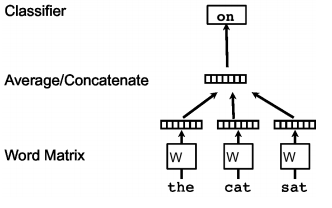
\includegraphics[height=0.2\textheight]{img/word2vec_skip_gram}
    \caption{Word2vec -- Skip gram architecture\cite{doc2vec}}
    \label{fig:word2vec_skip_gram}
\end{figure}

Other things to mention:
\begin{itemize}
    \item show 2D projection of vectors
    \item $king + woman - man = queen$
\end{itemize}

\subsection{Paragraph Vector (Doc2Vec)}
Explain doc2vec\cite{doc2vec}.

\begin{comment}
dbow
is a simpler model and ignores
word order, while
dmpv
is a more complex model
with more parameters

dbow 
works in the same way as skip-gram, except that the input is replaced by a special token representing the document (i.e. v_w_I is a vector rep-
resenting the document).  In this architecture, the order of words in the document is ignored; hence the name distributed bag of words.

dmpv
works in a similar way to cbow. For the input, dmpv introduces  an  additional  document token  in  addition  to  multiple  target  words. Unlike cbow, however, these vectors are not summed but concatenated (i.e.
v_w_I is a concatenated vector containing the document token and several target words). The objective is again to predict a context word given the concatenated document and word vectors..

\end{comment}

\begin{itemize}
    \item distributed memory version (dm) (\cref{fig:doc2vec_dm})
      \subitem small extension to cbow word2vec
      \subitem acts as a memory - what is missing from the current context?
    \item distributed bag of words (dbow) (\cref{fig:doc2vec_dbow})
      \subitem similar to skip-grams in word2vec
\end{itemize}

\begin{figure}[h]
	\centering
	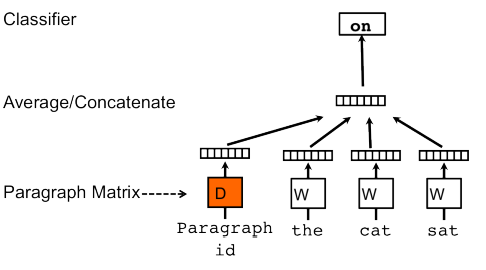
\includegraphics[height=0.2\textheight]{img/doc2vec_dm}
    \caption{Paragraph Vector -- Distributed Memory version\cite{doc2vec}}
    \label{fig:doc2vec_dm}
\end{figure}

\begin{figure}[h]
	\centering
	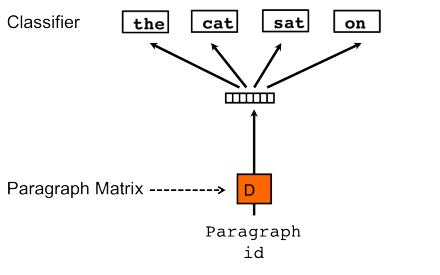
\includegraphics[height=0.2\textheight]{img/doc2vec_dbow}
	\caption{Paragraph Vector -- Distributed Bag of Words version\cite{doc2vec}}
	\label{fig:doc2vec_dbow}
\end{figure}

\subsection{Deep Learning}
deep learning\cite{Goodfellow}

Input - sequence of word embeddings.

\subsubsection{Recurrent Neural Network (RNN)}
\begin{itemize}
    \item cite relevant papers
    \item put an image of the network
    \item LSTM units
\end{itemize}

\subsubsection{Convolutional Neural Networks}
Show Yoon Kim's\cite{yoon_kim} architecture (\cref{fig:cnn_kim}).


Mention Zhang.\cite{cnn_zhang}.

\begin{figure}[h]
	\centering
	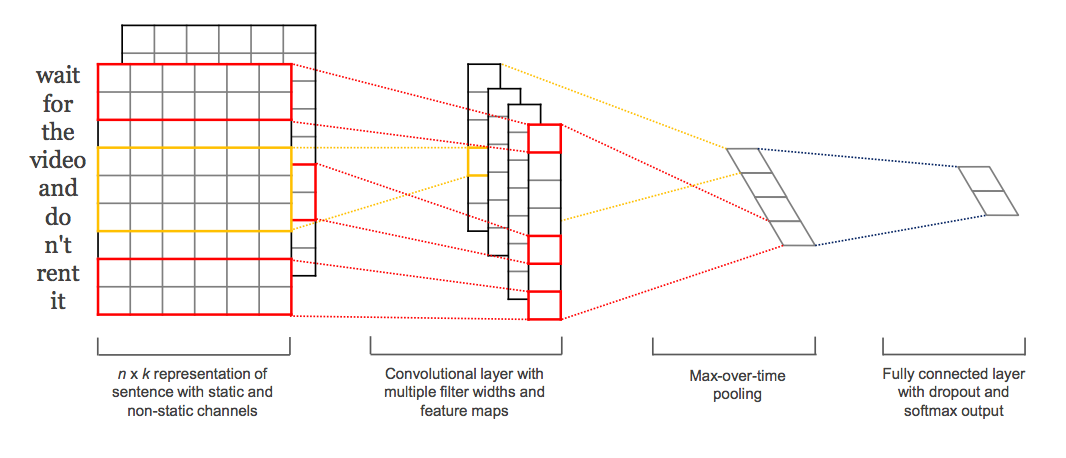
\includegraphics[height=0.2\textheight]{img/cnn_kim}
	\caption{Convolutional neural network with multiple filter sizes\cite{yoon_kim}}
	\label{fig:cnn_kim}
\end{figure}


%%%%%%%%%%%%%%%%%%%%%%%%%%%%%
%%%%%%%%% BOOSTING %%%%%%%%%%
%%%%%%%%%%%%%%%%%%%%%%%%%%%%%
\begin{comment}

\begin{itemize}
    \item Random Forest
    \item XGBoost
    \item stacking
\end{itemize}
\end{comment}



\begin{comment}
\subsection{Annoy}
Annoy\cite{annoy} is a algorithm developed by Erik Bernhardsson at Spotify, which enables quick search for the nearest neighbours. The drawback of the traditional kNN algorithm is its linear prediction time and huge amount of memory needed, which doesn't scale once we have hundreds of thousands data points.

Annoy uses random projections and recursively splits the space between two data points by a random hyperplane. All the splits are stored in the tree. The whole algorithm is run $n$ times to create $n$ trees. The more trees, the better the accuracy and slower the training and prediction time.
\end{comment}

\section{Project Gutenberg}
\begin{itemize}
    \item What is Project Gutenberg.
    \item How many books are there in Project Gutenberg
    \item What types (classes) of books
    \item Metadata for genre classification.
\end{itemize}

\chapter{Methodology}
In this chapter, we introduce the conducted experiment. After describing the dataset creation, we go into detail on the particular usage of text representation techniques and classification algorithms introduced in \cref{text_analysis} and \cref{classification_algorithms}.

\section{Dataset}
There are already some widely known datasets for text classification, such as the IMDB movie review dataset for sentiment analysis\cite{imdb_dataset} or datasets for various tasks in the UCI Machine Learning Repository\cite{UCI}. Nevertheless, we haven't found any publicly accessible dataset containing short text snippets of books. Therefore, we created a dataset out of the books available in Project Gutenberg. As the focus of our work is to recognize genres based on a short text, we cut several snippets out of each book of interest.

\subsubsection{Genres}
We rely on the \textit{subjects} tag in the Project Gutenberg metadata catalogue to determine genres of the books. After some cleaning (e.g. merging \textit{adventure} and \textit{adventure stories} together), we focused on texts belonging to one of the following genres:
\begin{itemize}
  \item adventure stories
  \item biography
  \item children literature
  \item detective and mystery stories
  \item drama
  \item fantasy literature
  \item historical fiction
  \item love stories
  \item philosophy and ethics
  \item poetry
  \item religion and mythology
  \item science fiction
  \item short stories
  \item western stories
\end{itemize}

We selected $5602$ distinct Project Gutenberg books containing one of the above defined genres. We didn't choose books covering multiple genres as the majority of classifiers is suited for a single class predictions. Also we would have to use more complex metrics to compare multiclass classification models.

Out of the $5602$ books, we sampled text snippets with the length of $3200$ characters. The whole dataset consisting of $225134$ documents was then split into train ($85\ \%$) and test set ($15\ \%$).

The original book texts were first preprocessed to get rid of the Project Gutenberg header and footer. After that, another $10000$ characters were stripped out of the beginning and end of the book to avoid book contents, preface or glossary being part of the document. Sequences of whitespace characters were replaced by a single space character as long whitespace sequences would bloat the documents with non-meaningful symbols.

Finally, in case the original book text was split in the middle of a word, the incomplete heading and trailing word of the document is discarded, which makes the documents slightly shorter than $3200$ characters.


\subsubsection{Document size}
As one of the main goals is to find out how much text is needed to distinguish a genre, we created two other datasets containing $800$ and $200$ characters long documents. The shorter datasets were created by taking first $n$ characters of the original dataset with $3200$ characters.\footnote{And again, discarding the last word in case the word was not complete.} These three document lengths approximately represent:
\begin{itemize}
  \item a snippet of few sentences ($200$ chars)
  \item a paragraph ($800$ chars)
  \item a couple of pages ($3200$ chars)
\end{itemize}
As the sizes are defined in characters and not words, the word count varies between documents.


\section{Genre Classification}

\begin{itemize}
  \item mention different tokenizing approaches
\end{itemize}

\begin{comment}
  For each document size, we explore three document representations. Bag of words creates a vector based on the occurrence of words in vocabulary, doc2vec approach encodes the document in a vector in several hundred dimensional space. Finally, we use GloVe word-embeddings as an input to the Convolutional Neural Network.
\end{comment}

\subsection{Bag of Words}
First, we represent documents as bag of words. One of the drawbacks of BOW is that it creates vectors in highly-dimensional space. That might cause problems in training as the whole dataset might not fit into memory or it can take very long time until some classifiers, for example SVMs, converge.

To see how many distinct words are needed in the BOW vector for a good prediction, we consider various vocabulary sizes from $1000$ to $50000$ words and compare performance of the classifiers for those.

When creating vocabulary with size $n$, the $n$ most frequent words which occur in less than $50\ \%$ of the documents are chosen. At the same time, chosen words most appear at least in $5$ documents to be considered at all. Filtering of the frequent words is more or less equivalent to stop word exclusion. By filtering the low occurrence words, we make sure that words such as names very specific to a given book are not included in the dictionary.


\subsubsection{Binary BOW}
Algorithms:
\begin{itemize}
  \item Naive Bayes
  \item Logistic Regression
  \item Feed-Forward NN
\end{itemize}

\subsection{Doc2Vec Representation}
We use the DBOW version of doc2vec algorithm. The parameter choice was inspired by \cite{doc2vec_params}, who ran grid search comparing various settings on a task with document sizes similar to ours.

For the doc2vec representation, we compared following algorithms:
\begin{itemize}
  \item most similar genre vector
  \item Gaussian Naive Bayes
  \item Logistic Regression
  \item Feed-forward NN
  \item Annoy
\end{itemize}

\chapter{Data Exploration}


In the following, we explore some elementary properties of the $225134$ documents in our dataset. The linguistic properties are made on the full-length documents ($3200$ characters).

\subsubsection{Genre Distribution}

\begin{figure}[h]
	\centering
	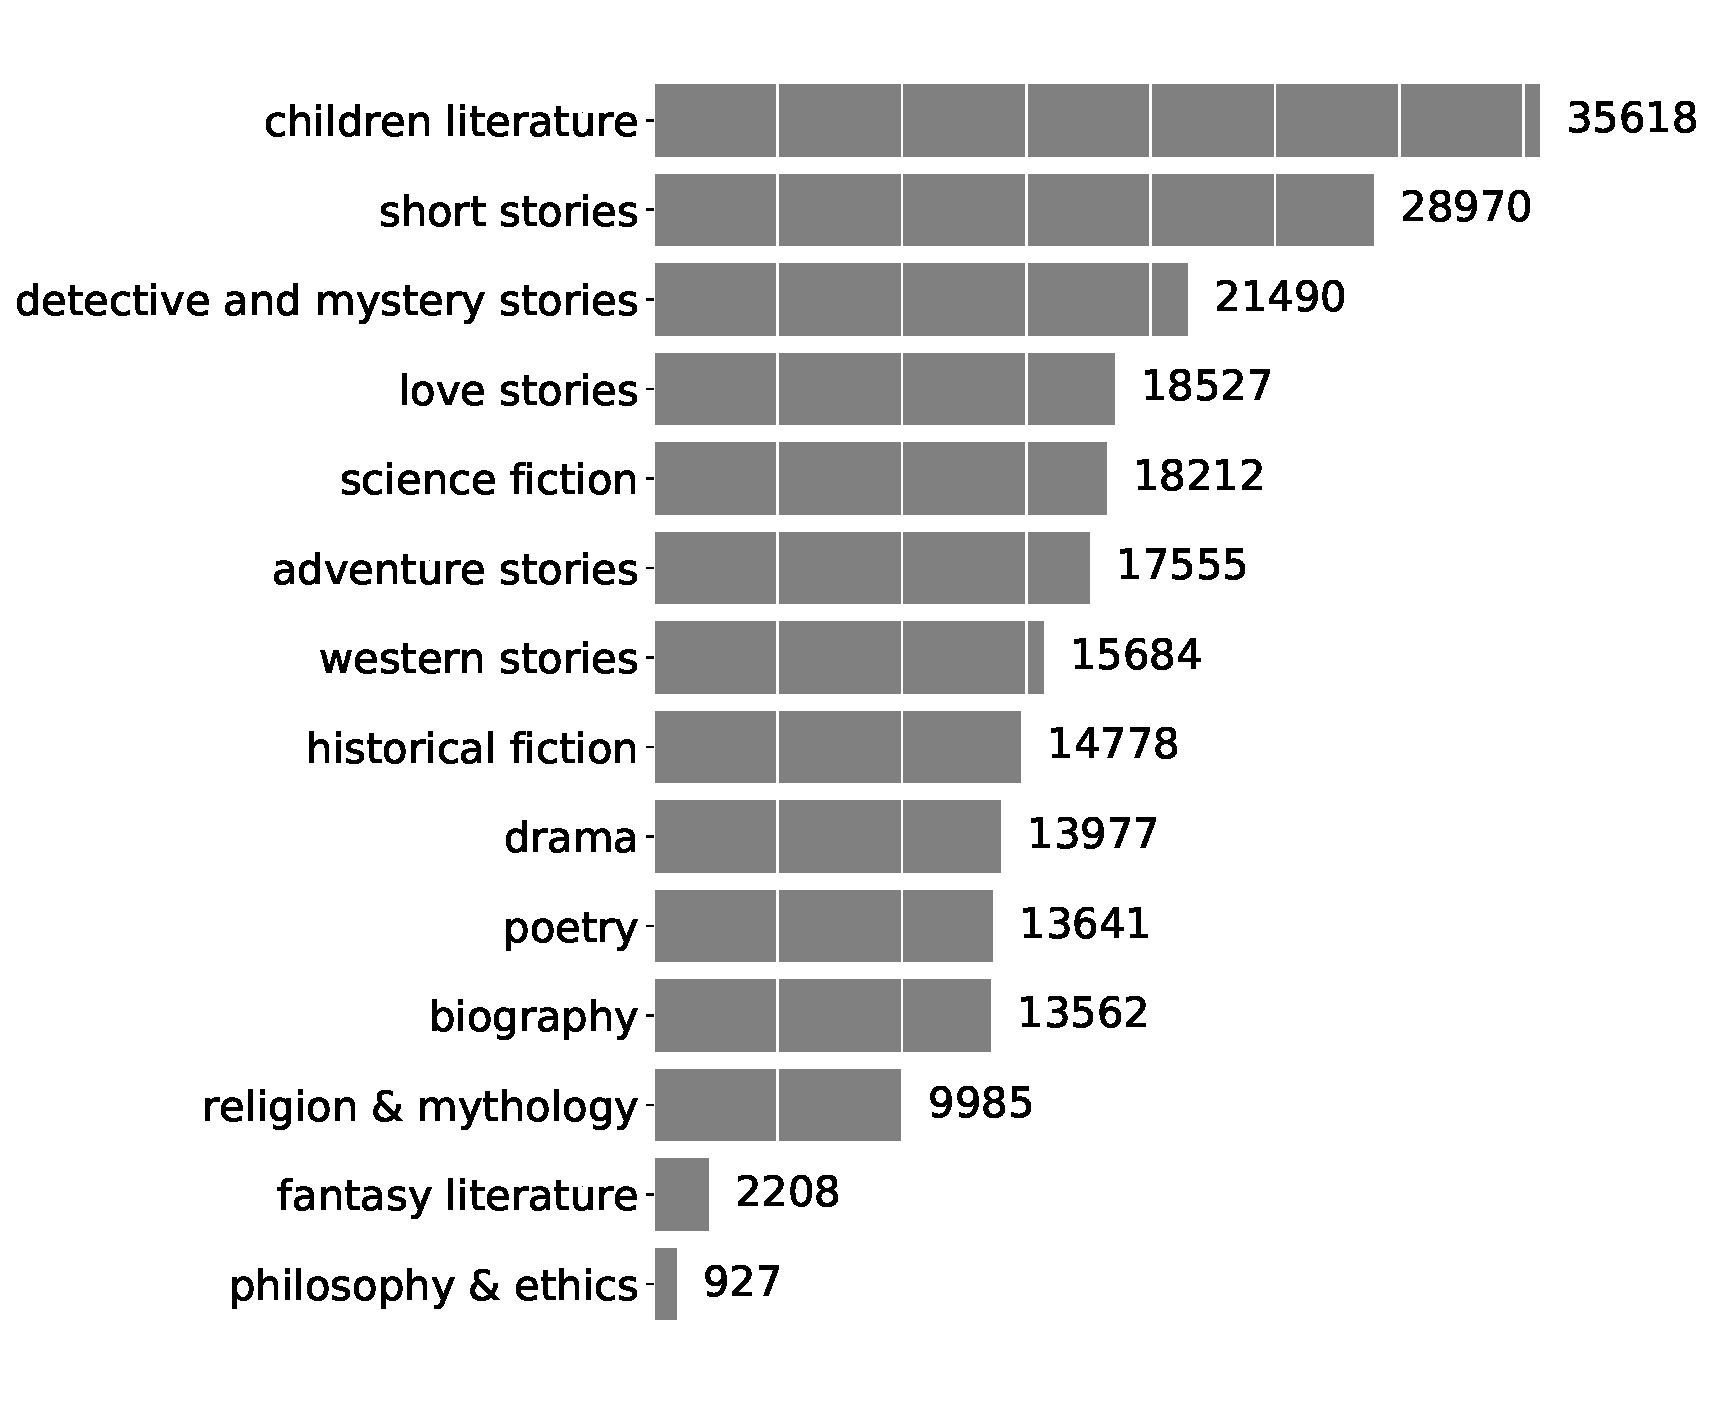
\includegraphics[height=0.4\textheight]{img/03_01_genre_distribution}
	\caption{Genre distribution among documents.}
	\label{fig:genre_distribution}
\end{figure}




\begin{comment}

\subsubsection{Average Word Length}
\begin{itemize}
    \item How do we define word
    \item Distribution per genre
\end{itemize}
\begin{figure}[h]
	\centering
	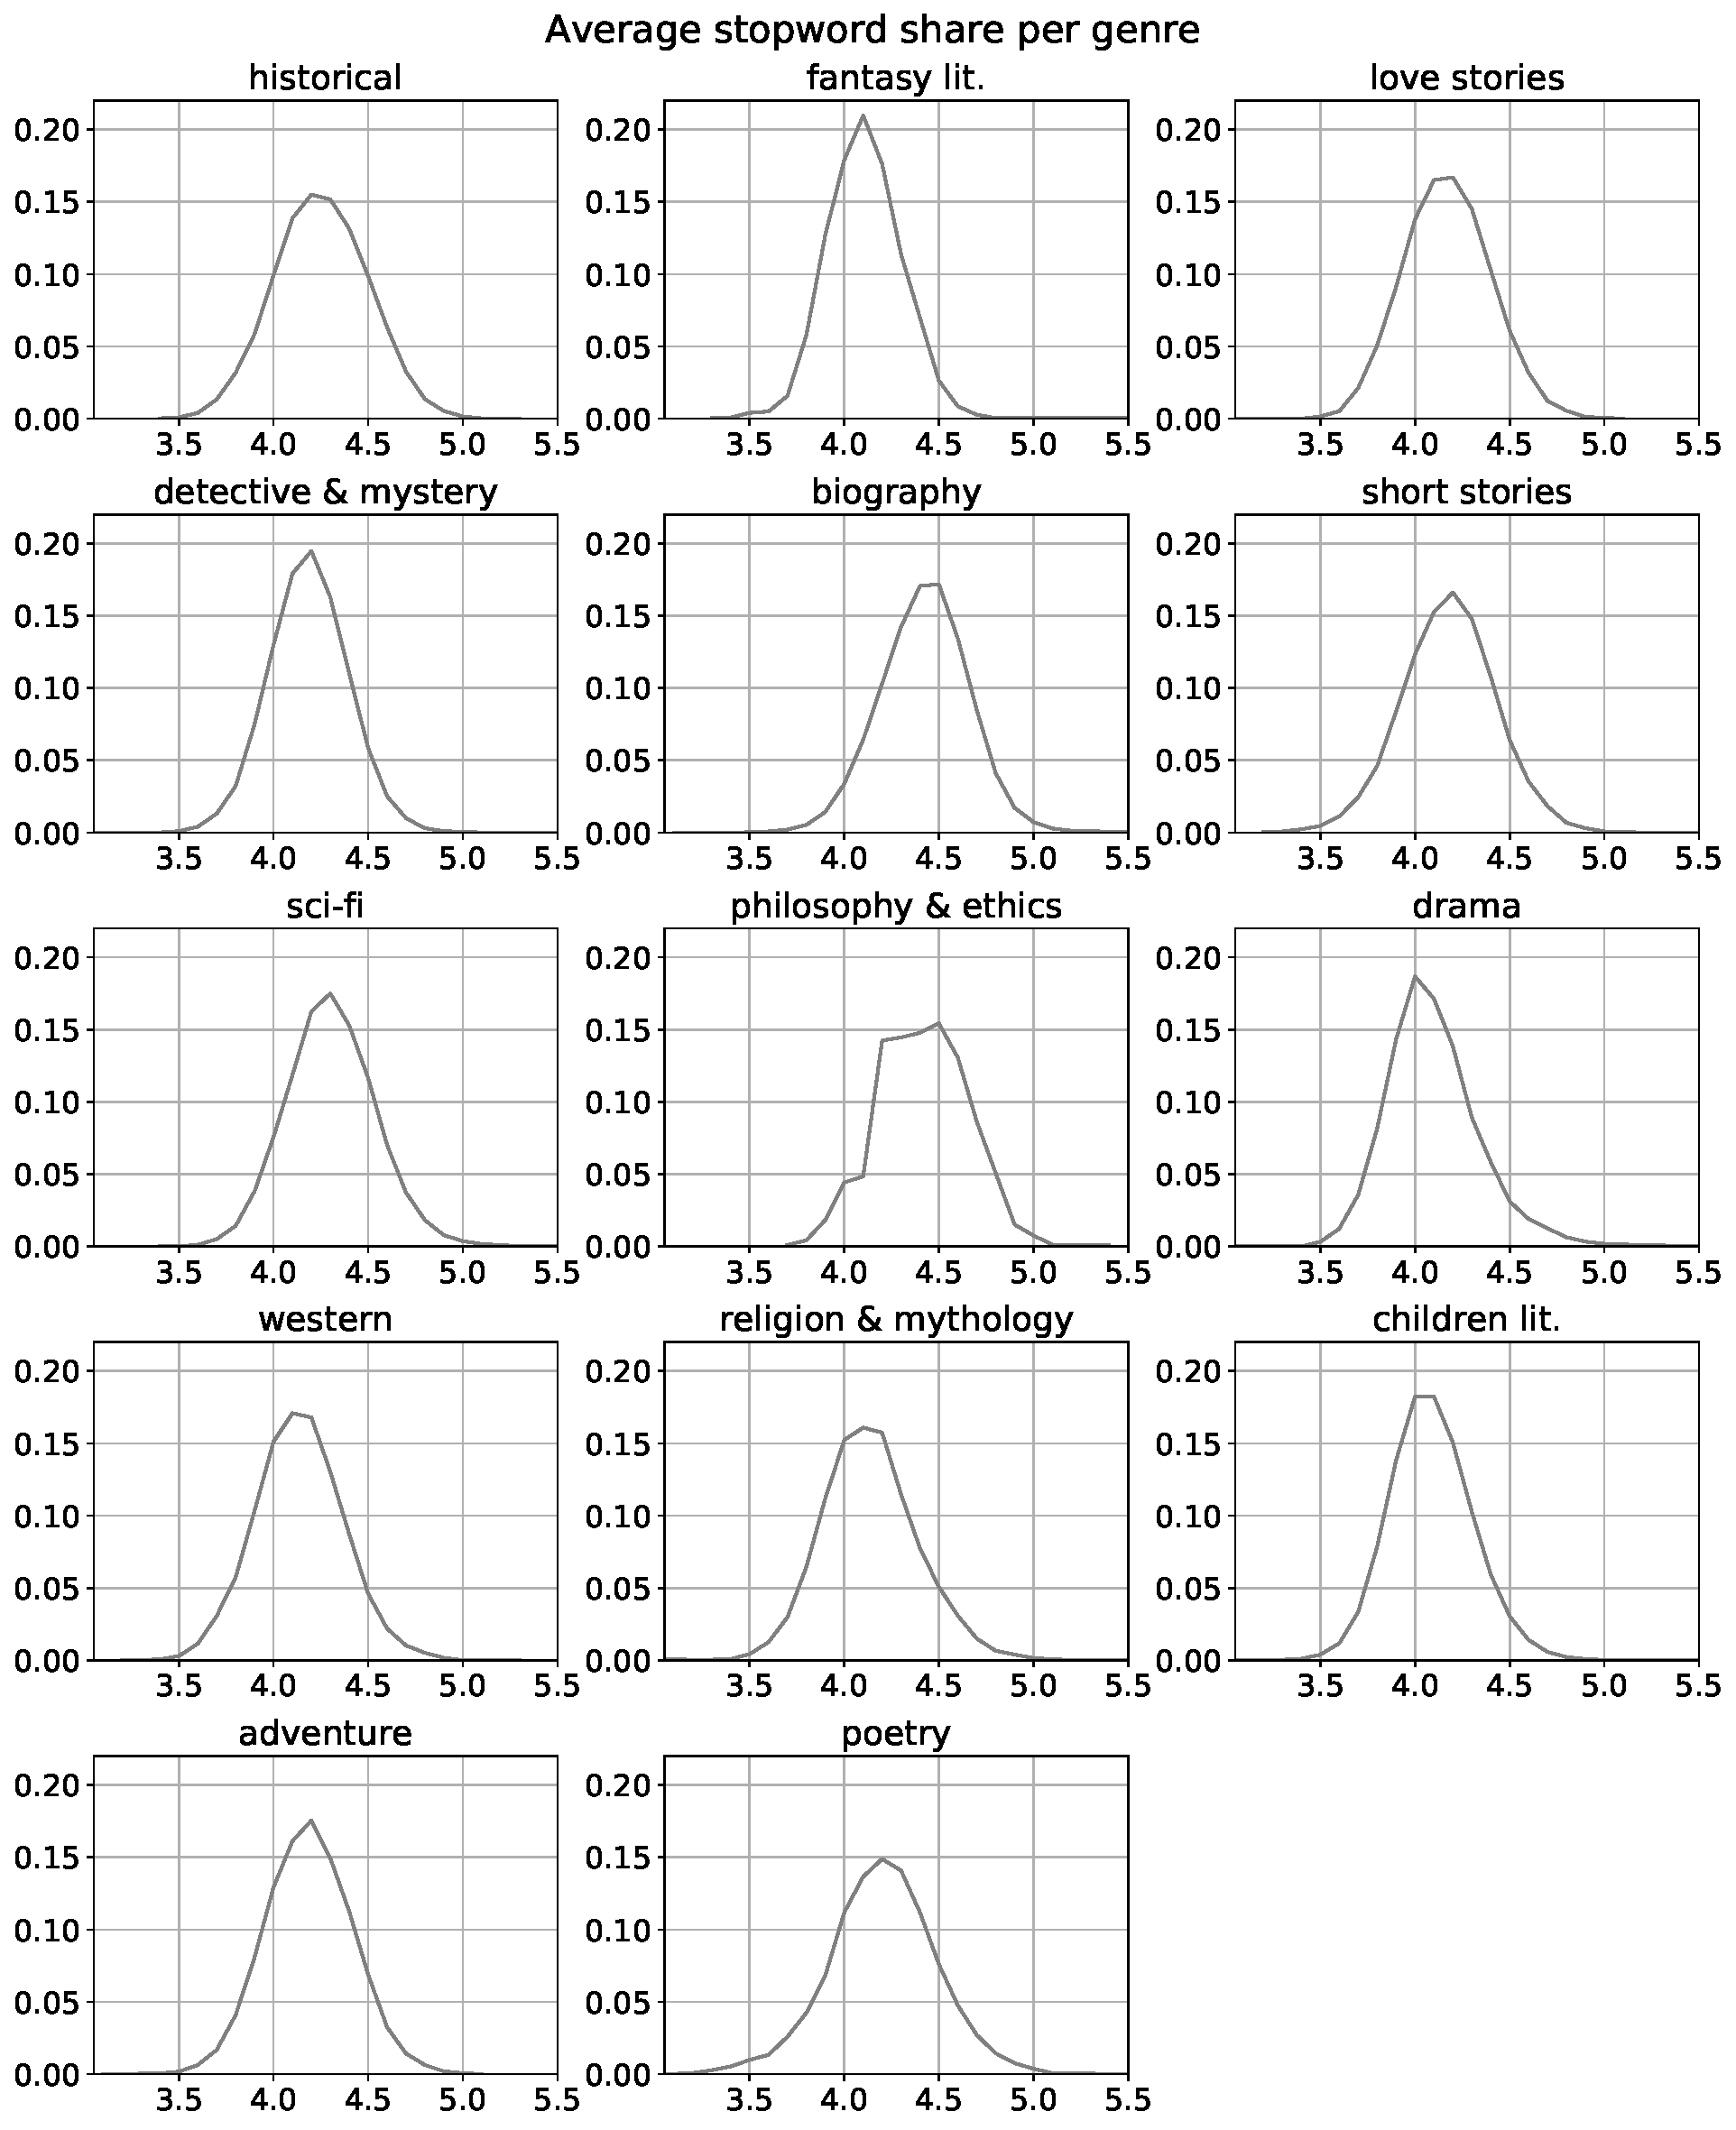
\includegraphics[height=0.4\textheight]{img/03_avg_word_length}
	\caption{Average word length per genre.}
	\label{fig:avg_word_length}
\end{figure}

%%%%%%%%%%%%%%%%%%
%%% SUBFIGURES %%%
%%%%%%%%%%%%%%%%%%

\begin{figure}
\centering

\begin{subfigure}[t]{.5\textwidth}
	\centering
	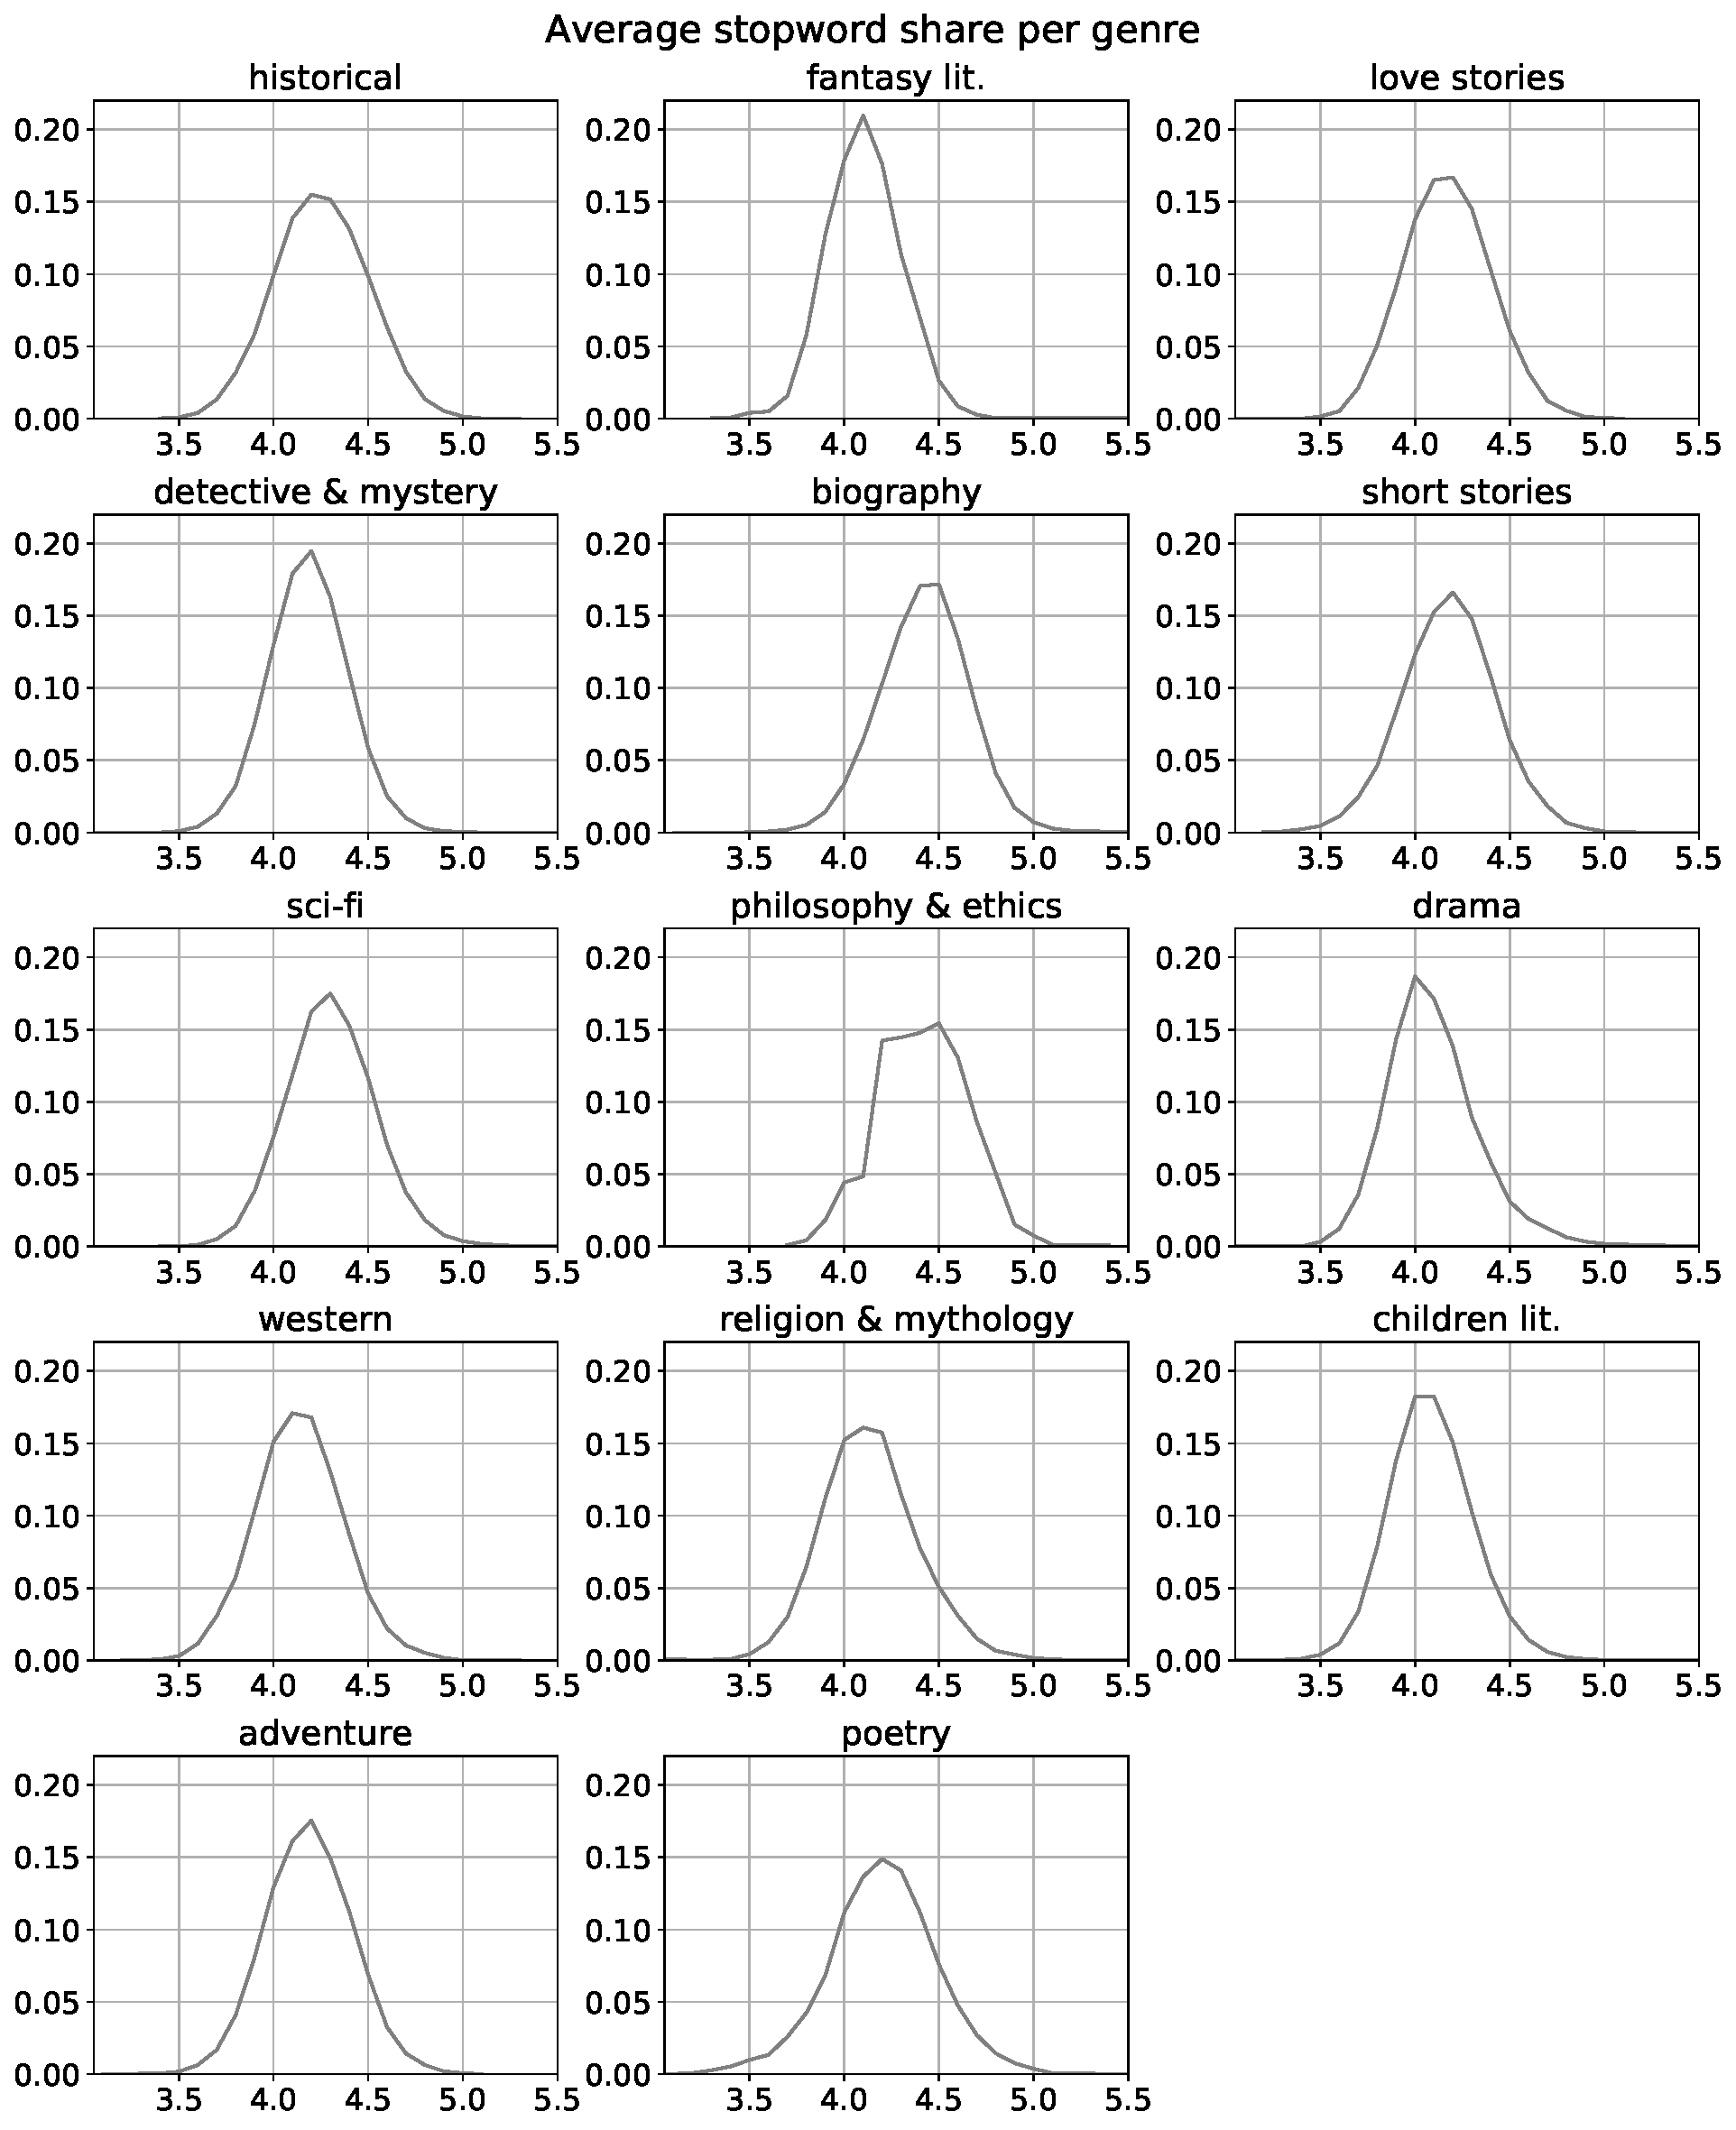
\includegraphics[width=.95\linewidth]{img/03_avg_word_length}
	\caption{Average word length per genre.}
	\label{fig:avg_word_length}
\end{subfigure}%
\begin{subfigure}[t]{.5\textwidth}
	\centering
	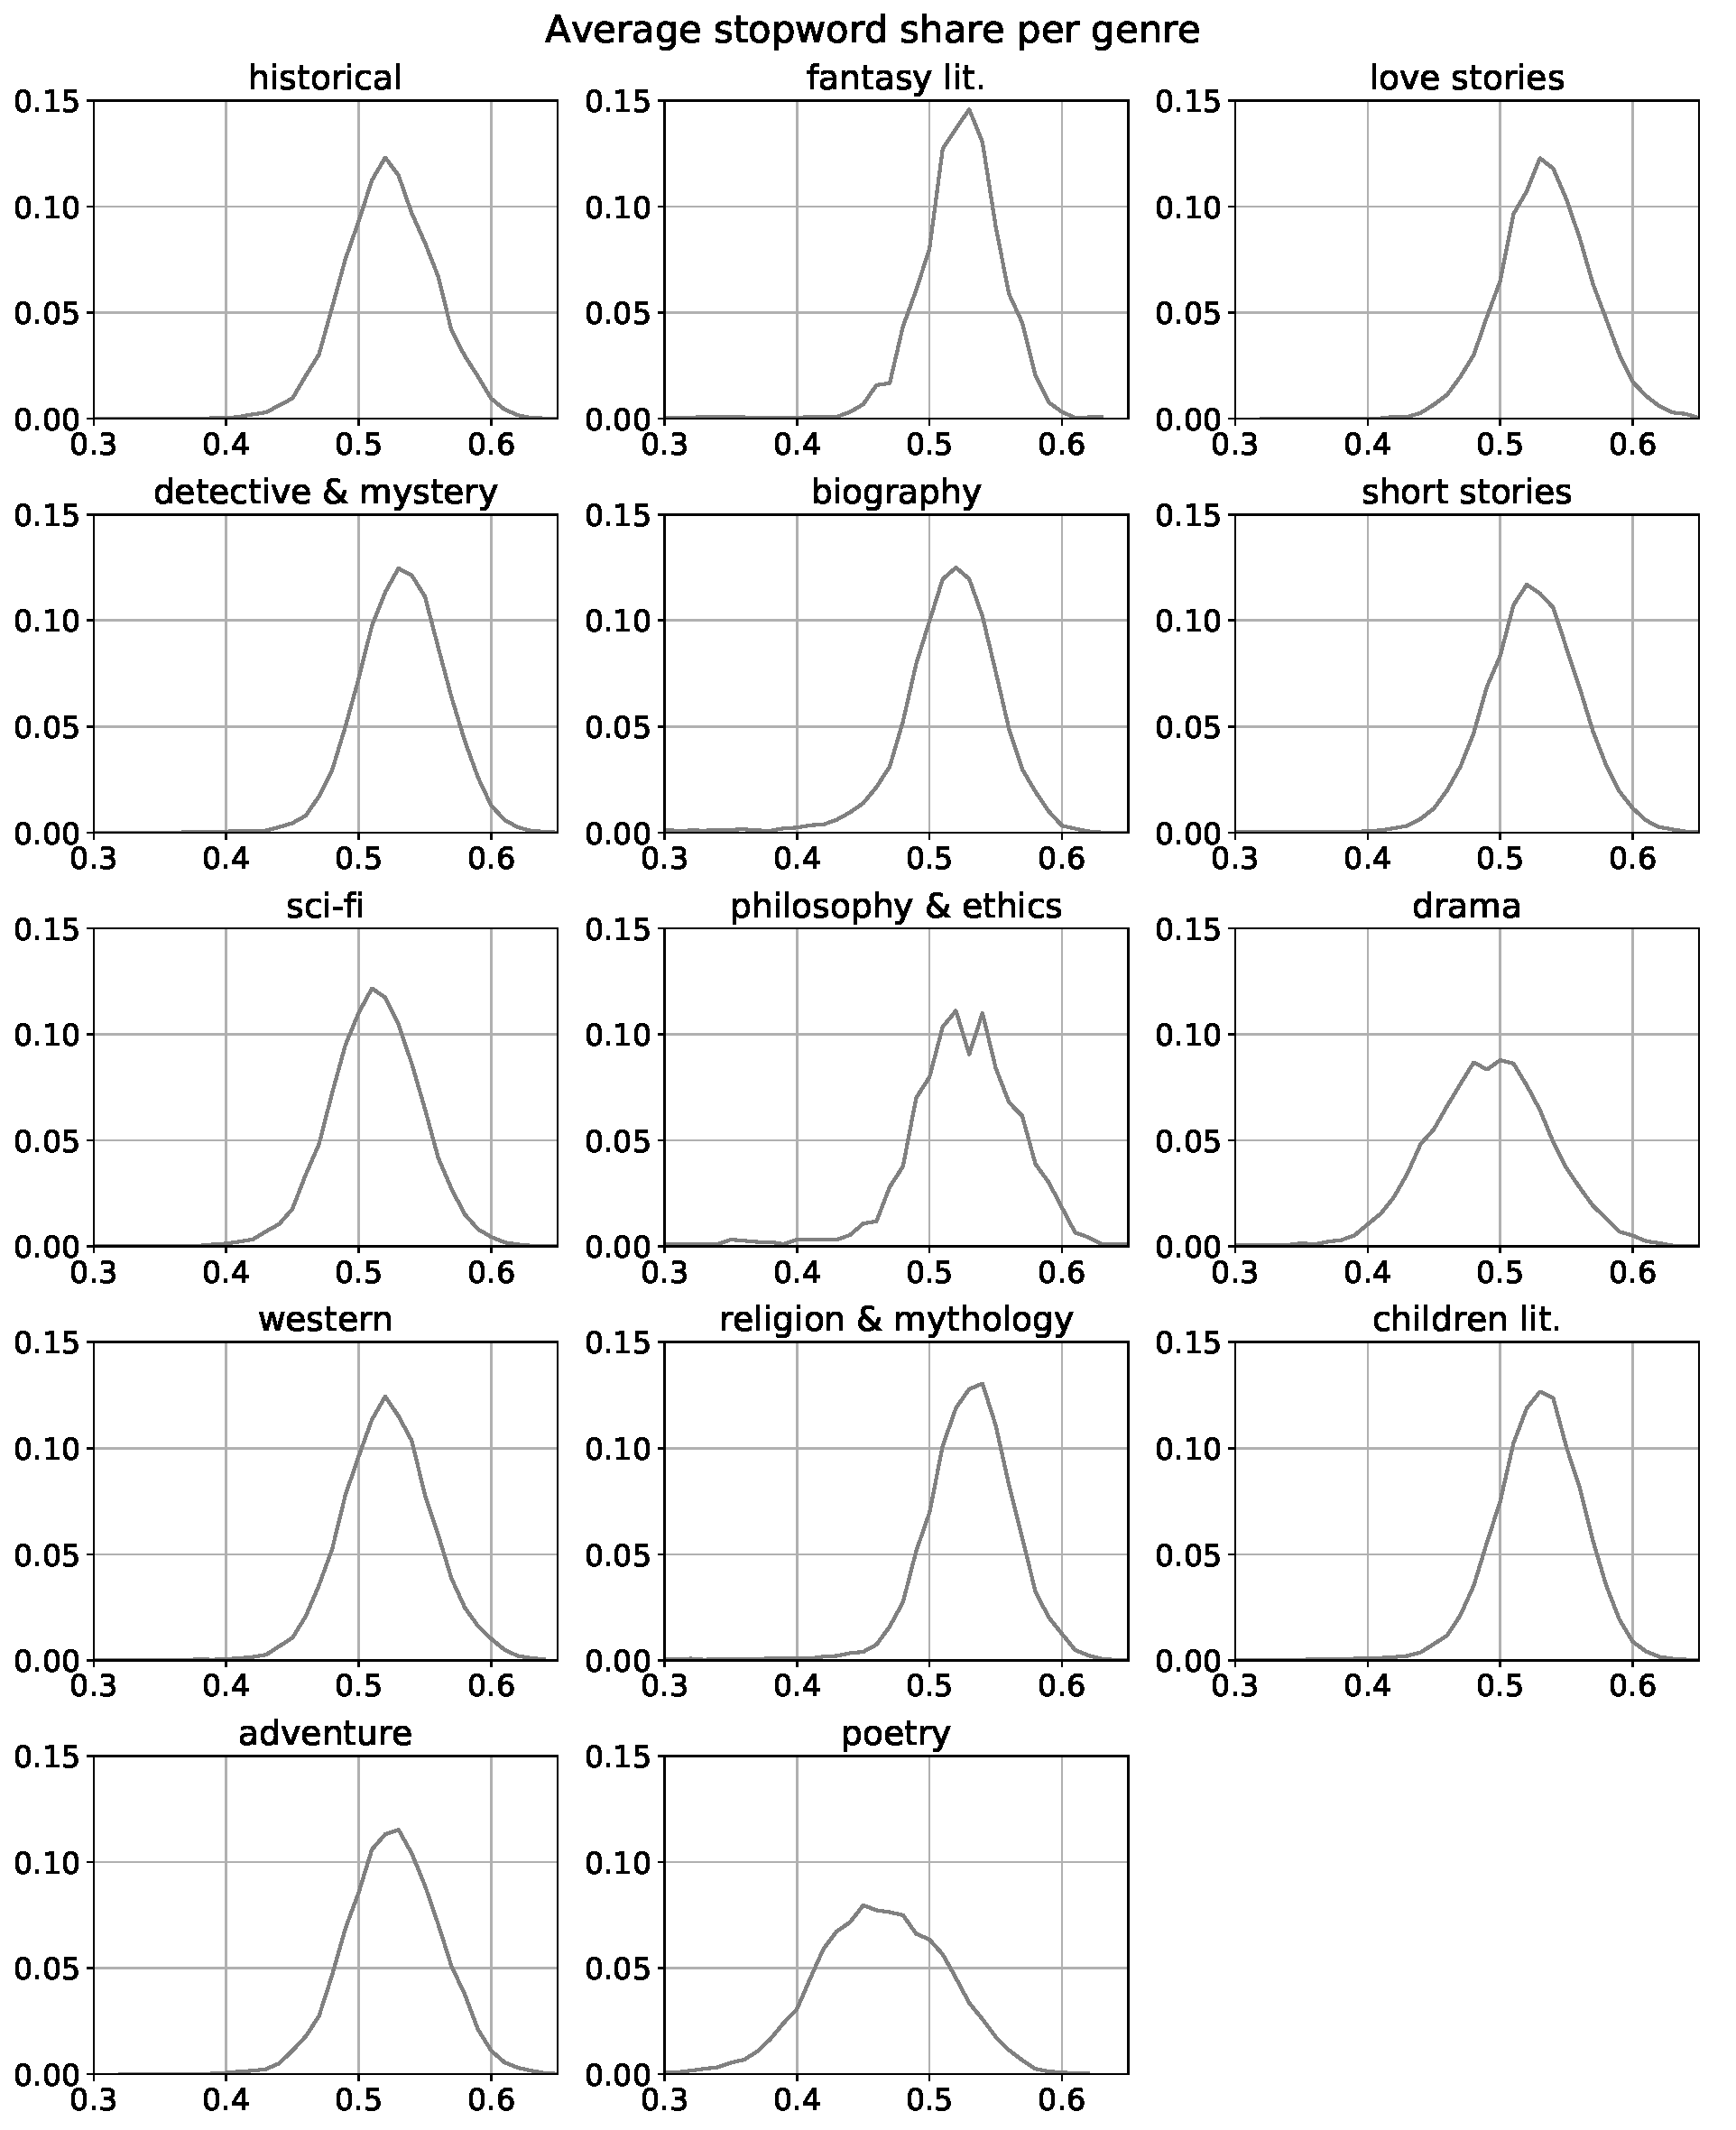
\includegraphics[width=.95\linewidth]{img/03_stopwords}
	\caption{Average stopwords share per genre.}
	\label{fig:stopwords}
\end{subfigure}
\caption{X}
\end{figure}


\end{comment}




\begin{comment}
\begin{tabular}{cc}
  Table head & Table head\\
  Some values & Some values\\
  Some values & Some values\\
  Some values & Some values\\
  Some values & Some values\\
\end{tabular}
\end{comment}

\begin{comment}
\subsubsection{Author Distribution}
\begin{itemize}
    \item How many authors
    \item Snippets per author distribution
    \item Main authors
\end{itemize}

\subsubsection{Average Sentence Length}
\begin{itemize}
    \item How do we define sentence
    \item Distribution per genre
\end{itemize}
\end{comment}
% Readability measures - https://pypi.org/project/ReadabilityCalculator





\begin{comment}


\subsubsection{Stop Words Proportion}
Stop words definition as in \texttt{nltk.corpus.stopwords}. Examples of what stopwords are in.
\begin{figure}[h]
	\centering
	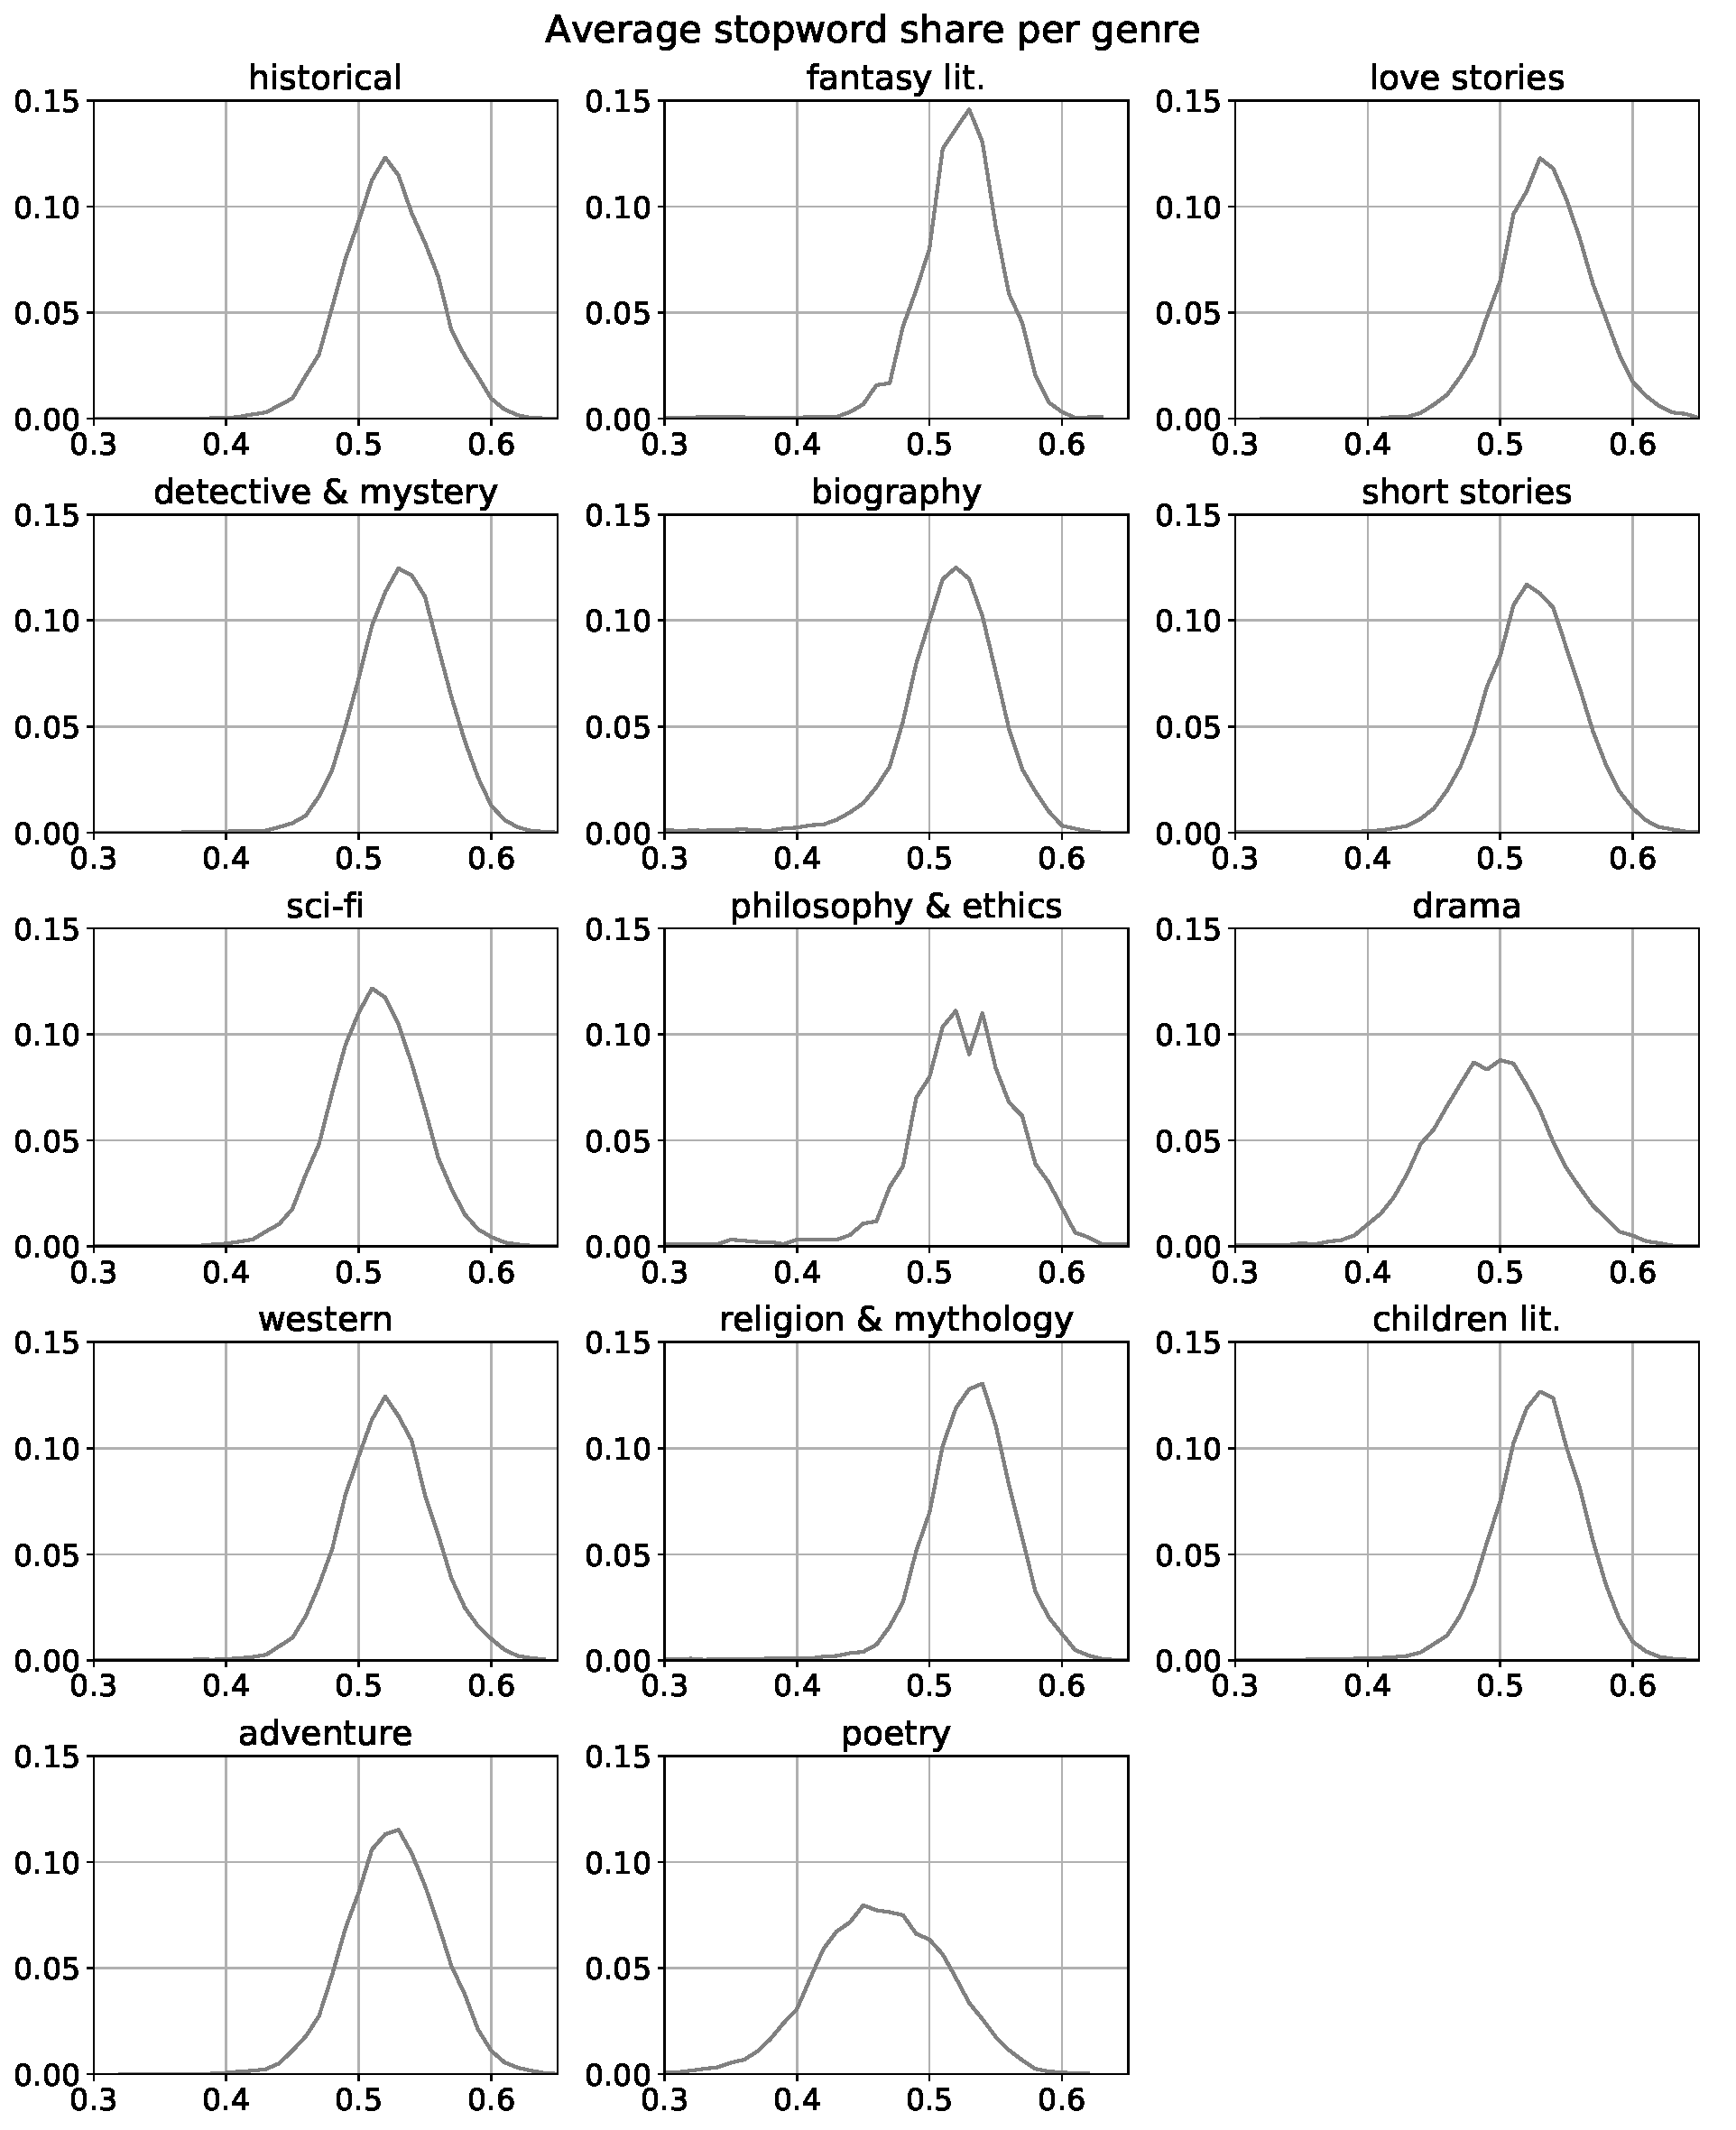
\includegraphics[height=0.4\textheight]{img/03_stopwords}
	\caption{Average stop words share per genre.}
	\label{fig:stopwords}
\end{figure}

\end{comment}



\begin{comment}
\subsubsection{Part of speech}
\end{comment}

\chapter{Evaluation}

In this chapter, we compare various classifiers for each document representation and discuss the choice of hyperparameters.

For both \textit{BOW} and \textit{doc2vec} document representation, we first show the performance for each classifier individually. The classifier is trained on three lengths of documents -- $200$, $800$ and $3200$ characters. The goal is to see how much better (if at all) is the score for longer documents. At the end of both BOW and doc2vec sections we compare all classifiers for that representation. Finally, we compare both representation and created a combined model using both approaches.


\subsection{Evaluation metric}
As the classes are not balanced (there are $35618$ documents in \textit{children literature} class and only $927$ in \textit{philosophy and ethics}), we will not optimize accuracy but \textit{F1-macro} score, which is defined as:
$$ F_1 = \frac{2PR}{P+R}$$
where $P$ and $R$ are precision and recall averaged over all classes $C_i \in C$ with equal weight\footnote{Which means a misclassification in smaller classes changes the score more than a misclassification in bigger ones.}.

$$P = \frac{1}{|C|}\sum_{i=1}^{|C|}P_i$$
$$R = \frac{1}{|C|}\sum_{i=1}^{|C|}R_i$$

$P_i$ and $R_i$ are then standard precision and recall defined for single class $i$:
$$P_i = \frac{TP_i}{TP_i + FP_i}$$
$$R_i = \frac{TP_i}{TP_i + FN_i}$$

where $TP_i$, $FP_i$ and $FN_i$ are number of true positive, false positive and false negative prediction for class $i$.

\textit{Precision} describes how often was the classifier right when predicting class $i$. \textit{Recall}, on the other hand, captures how often did the classifier predicted class $i$ for documents of class $i$.

To illustrate the computation of the F1-score with \textit{macro} weighting, we compute the test set score for a baseline class predictor which blindly predicts the majority class for every document:
\begin{itemize}
	\item $33771$ documents in the test set
	\item $14$ genres in total
	\item the majority class is \textit{children literature} with $5314$ occurrences
\end{itemize}

For all genres $g$ except for \textit{children literature}, the true positive rate $TP_g$ is equal to $0$ as the predictor never classifies a document in that class. That means that precision $P$ and recall $R$ for those classes is $0$.

For \textit{children literature} class the precision and recall are

\begin{equation}
	\begin{split}
		P_{children\ literature} & = \frac{5314}{33771} = 0.1574 \\
		R_{children\ literature} & = \frac{5314}{5314 + 0} = 1
	\end{split}
\end{equation}

\begin{comment}
\begin{align*}
		P_{children\ literature} &= \frac{5314}{33771} & &= 0.1574 \\
		R_{children\ literature} &= \frac{5314}{5314 + 0} & &= 1
\end{align*}
\end{comment}

as there was no children literature document that was misclassified.

With macro weighting, we get overall precision and recall as 
\begin{equation}
	\begin{split}
	P  & = \frac{1}{14}(13 \cdot 0 + 1 \cdot 0.1574)  = 0.0112 \\
	R & = \frac{1}{14}(13 \cdot 0 + 1 \cdot 1)   = 0.0714
	\end{split}
\end{equation}

Finally, the F1-macro score is then
$$ F_{1-macro} =  \frac{2PR}{P+R} = \frac{2 \cdot 0.0112 \cdot 0.0714}{ 0.0112 + 0.0714} = 0.0194$$

The accuracy, on the other hand, would have been $\frac{5314}{33771} = 0.1574$ which is much higher than the F1-score as the metric does not take class sizes into account. To train the classifier to perform well on all $14$ classes, we optimize the F1-score and only report accuracy for comparison.


\section{Bag of Words}
First, we represent the documents as \textit{binary} bag of words and explore how does the vocabulary size influence the classification performance. As the time and space complexity of the model training are dependent on the size of vocabulary, we want to know if the added complexity brings boost in performance or if the models are overfitted on the training vocabulary. The performance is shown for vocabulary sizes from $1000$ words up to $50000$ words.

When limiting the vocabulary size to $n$ words, we select the $n$ most frequent words which appear in less than $50\ \%$ of all documents. These words also have to occur in at least $5$ distinct documents to be considered for the vocabulary at all. For short documents ($200$ characters, only score for vocabulary up to $30000$ words is shown as the performance stays constant for bigger vocabulary sizes. The reason for that is that if we filter out words occurring in less than $5$ documents, there are only ca. $32000$ words left.

In the following, we compare the classification performance of Naive Bayes classifier, Logistic Regression and feed-forward neural network with two hidden layers. 

\subsection{Naive Bayes}
The Naive Bayes classifier turned out to be a very decent model for the short documents where it reached the same result as logistic regression while having training time under 1 second\footnote{Training was done on a single core on a computer with 2.5 GHz Intel Core i7 CPU}. The performance of Naive Bayes classifier improved with increasing the vocabulary size as shown in \cref{fig:naivebayes}. However, the F1-score for short texts improved by less than $0.01$ when increasing the vocabulary size from $20000$ to $30000$. For middle-length texts, the score improved by only $0.001$ when increasing the vocabulary size from $40000$ to $50000$. 



The best F1-score and accuracy for all three document lengths are listed in \cref{tbl:naivebayes}.

\begin{figure}[h]
	\centering
	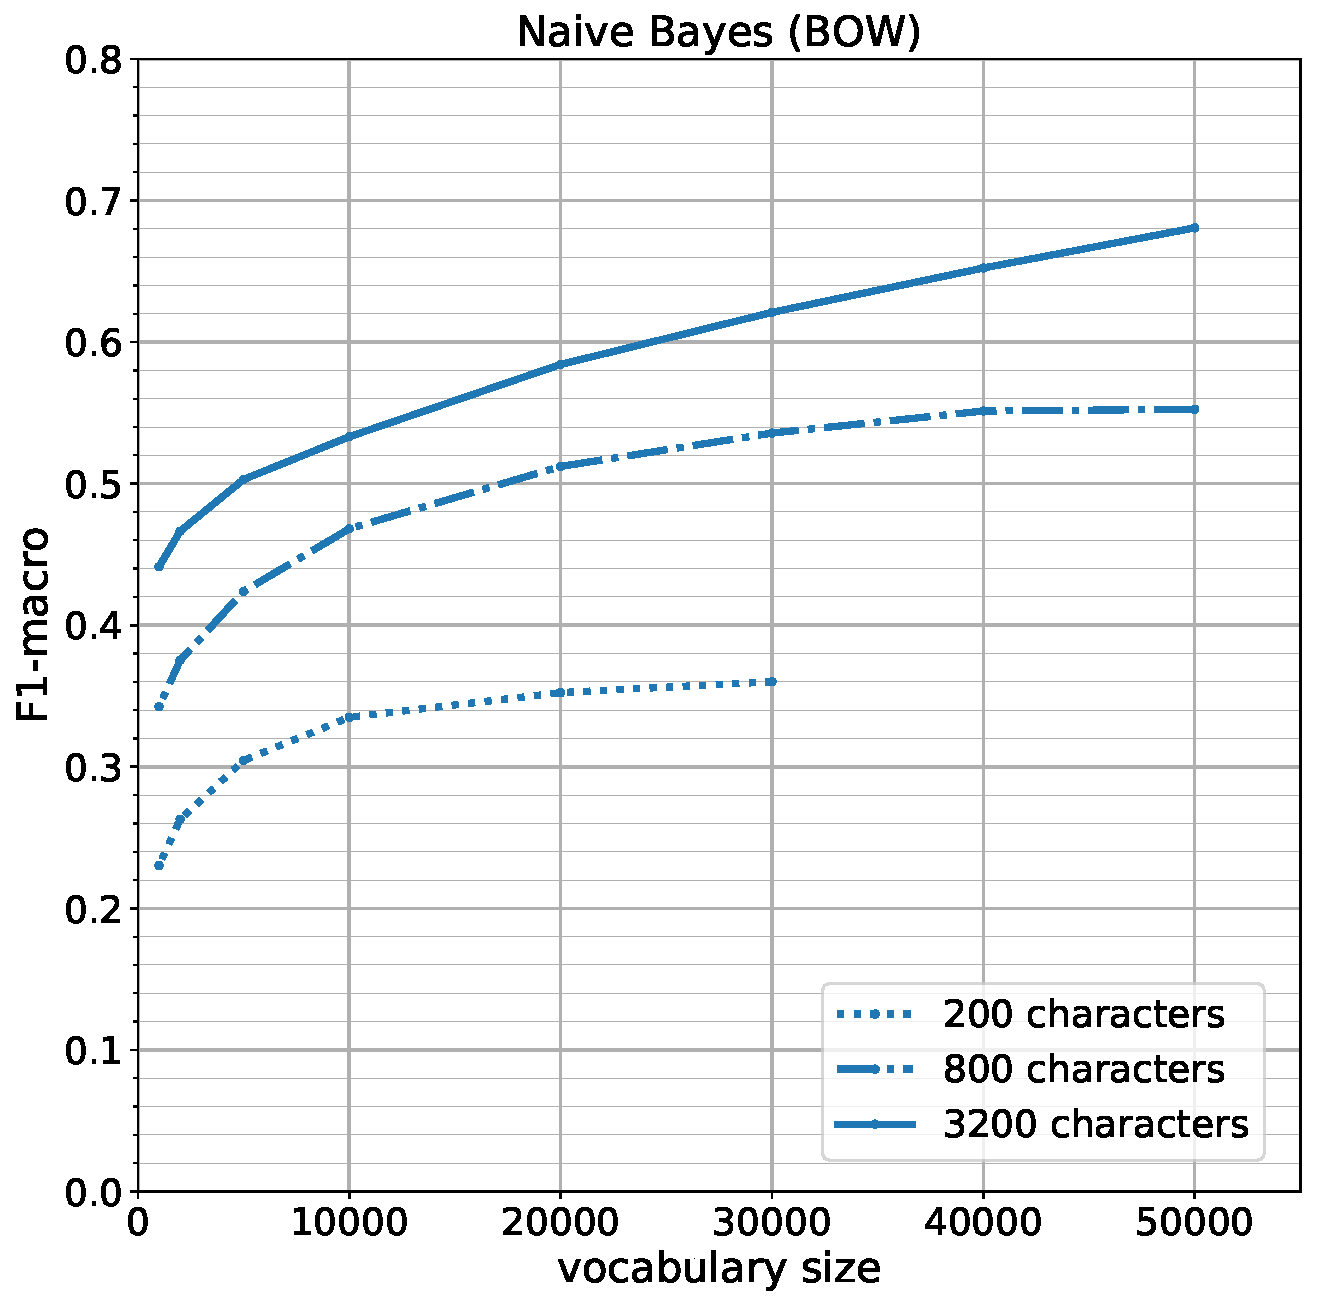
\includegraphics[height=0.3\textheight]{img/05_bow_nb}
	\caption{F1-macro score comparison for Naive Bayes based on text length and vocabulary size.}
	\label{fig:naivebayes}
\end{figure}

\begin{table}[h]
	\centering
	\begin{tabular}{|l|r|r|}\hline
		Document length (vocabulary size) & F1-macro score & Accuracy \\
		\hline
		$200$ chars ($30000$ words)    &   $0.360$      & $0.413$       \\
		$800$ chars ($50000$ words)     &  $0.553$   & $0.572$        \\
		$3200$ chars ($50000$ words)    &  $0.681$   & $0.678$    \\
		\hline
	\end{tabular}
	\caption{Best performance of \textbf{Naive Bayes} on \textbf{binary BOW} for each document length.}
	\label{tbl:naivebayes}
\end{table}


\begin{comment}
For short texts ($200$ characters), classifier reached F1-score $0.396$ and $0.418$ accuracy, for middle-length texts ($800$ characters) $0.571$ F1-score and $0.570$ accuracy. For the long texts of length $3200$ characters, F1-score for Naive Bayes reached $0.615$ and accuracy $0.613$.
\end{comment}

%%%%%%%%%%%%%%%%%%%%%%%%%%%%%%%%%%
%%%%% LOGISTIC REGRESSION %%%%%%%%
%%%%%%%%%%%%%%%%%%%%%%%%%%%%%%%%%%
\subsection{Logistic Regression}
Logistic Regression on binary BOW performed better than Naive Bayes for short and medium-length documents. \cref{fig:bow_logreg} shows the F1-scores for all tested vocabulary sizes and \cref{tbl:bow_logreg} lists best results of the Logistic Regression for each document length.

\begin{figure}[h]
	\centering
	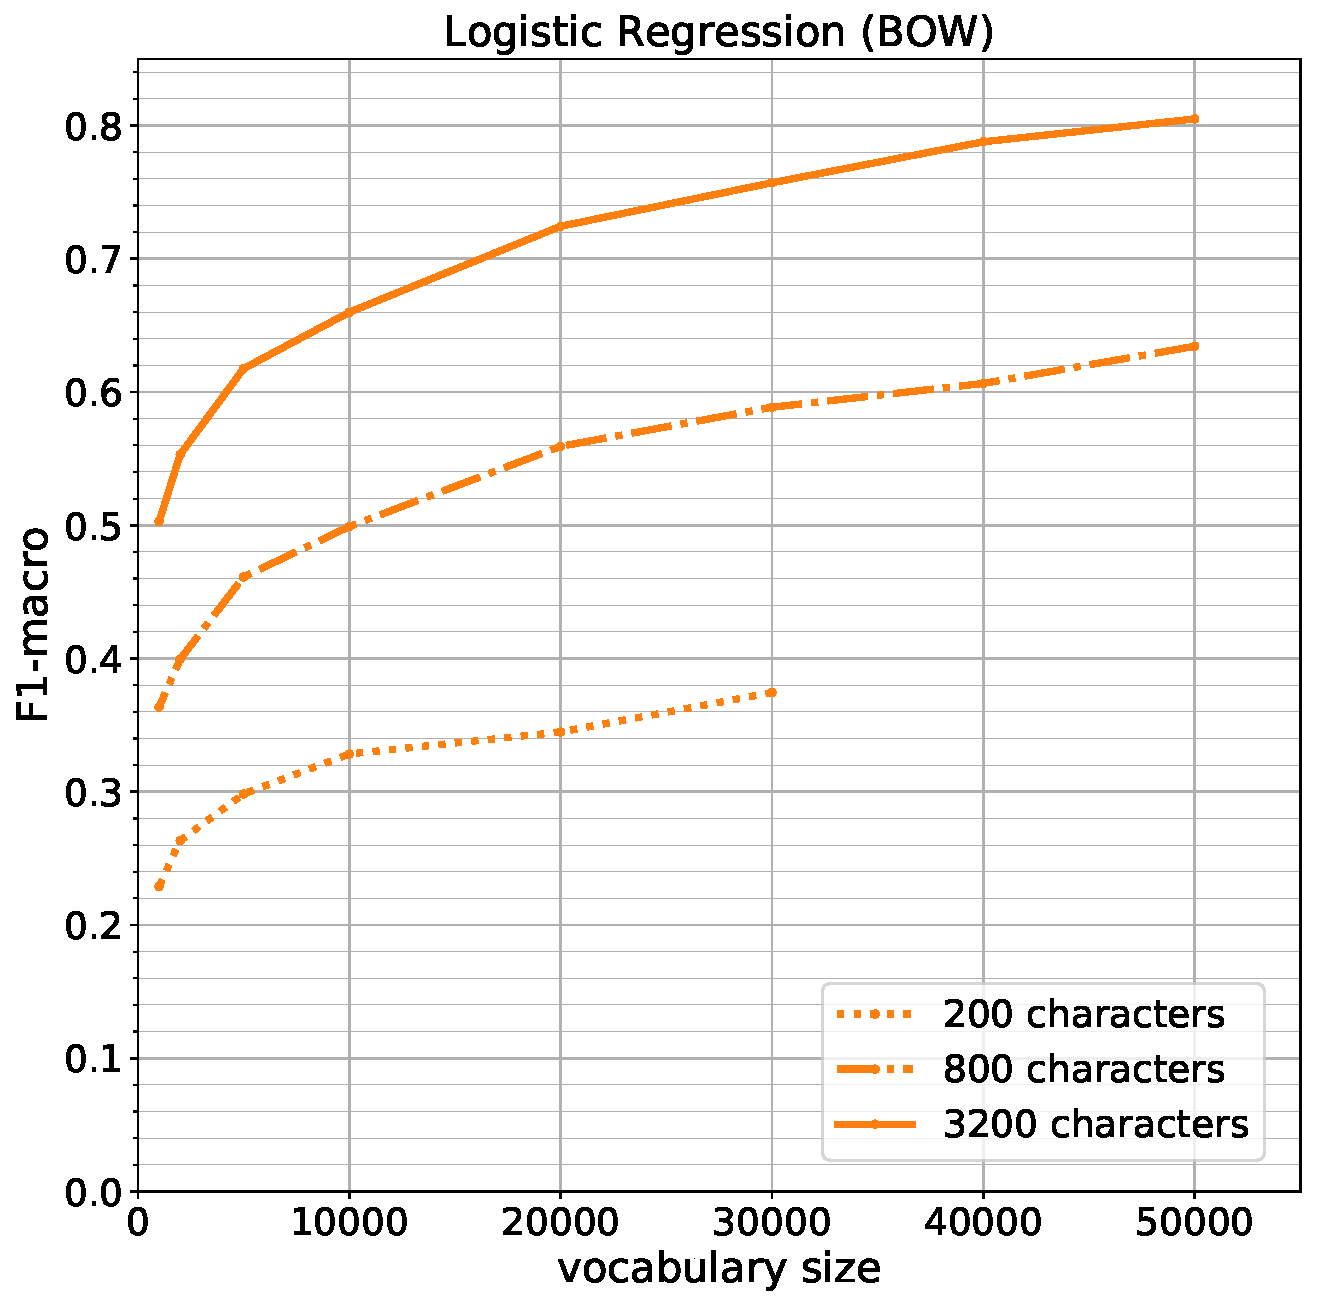
\includegraphics[height=0.3\textheight]{img/05_bow_logreg}
	\caption{F1-macro score comparison for Logistic Regression with binary BOW representation based on text length and vocabulary size.}
	\label{fig:bow_logreg}
\end{figure}

\begin{table}[h]
	\centering
	\begin{tabular}{|l|r|r|}\hline
		Document length (vocabulary size) & F1-macro score & Accuracy \\
		\hline
		$200$ chars ($30000$ words)    &   $0.374$   & $0.398$       \\
		$800$ chars ($50000$ words)     &  $0.634$   & $0.637$        \\
		$3200$ chars ($50000$ words)    &  $0.805$   & $0.802$    \\
		\hline
	\end{tabular}
	\caption{Best performance of \textbf{Logistic Regression} on \textbf{binary BOW} for each document length.}
	\label{tbl:bow_logreg}
\end{table}

For vocabulary size greater than $10000$, training with all $191363$ documents does not fit into $16$ GB of RAM. Therefore, we used \textit{sklearn}'s stochastic gradient descent with logistic loss which corresponds to logistic regression.

The best Logistic Regression classifier on binary BOW trained on long documents with vocabulary containing $50000$ words reached F1-score $0.805$ and accuracy $0.801$.

For each vocabulary size, \textit{grid search} was used to find the best regularization strength parameter $\alpha$. Generally, the optimal $\alpha$ value increased with document size and decreased with the size of vocabulary. The optimal $\alpha$ for the already mentioned best classifier was $0.0003$.


%%%%%%%%%%%%%%%%%%%%%%%%%%%%%%%%%%
%%%%% Feed-forward NN%%%% %%%%%%%%
%%%%%%%%%%%%%%%%%%%%%%%%%%%%%%%%%%
\subsection{Feed-forward NN}
Next classifier we tried out for the binary BOW representation was a simple feed-forward neural network with $2$ hidden layers of $200$ and $100$ neurons. We used \textit{ReLU} as an activation function for hidden layers, and \textit{softmax} on the output layer.

To decrease overfitting of the net, dropout layers were added between the layers with following coefficients:
\begin{itemize}
  \item $\textbf{0.4}$ between input and first hidden layer with $200$ neurons
  \item $\textbf{0.1}$ between first hidden layer with $200$ neurons and second with $100$ neurons
\end{itemize}
\cref{fig:bow_nn_architecture} shows the architecture of the net.

In \cref{fig:bow_nn} we can see that the F1-score of the feed-forward neural network improves with increasing vocabulary size as did the previous two algorithms. Even between the vocabulary size of $40000$ and $50000$, there is still about $0.02$ score difference.

The best F1-score reached for long documents was $0.849$ which is about $4\ \%$ better than the logistic regression. That comes as no surprise as logistic regression is equivalent to neural network with softmax output layer activation and no hidden layer.\footnote{except for regularization} As our net has two hidden layers, it is then computationally stronger than logistic regression. Best results also for shorter documents is shown in \cref{tbl:bow_nn}.

For long documents, the net overfitted massively the training data and reached accuracy score of $99\ \%$ on the training set. One way to deal with the overfit is to increase the dropout rate on the input layer. Another possibility is to decrease the number of neurons in the hidden layer. However, this kind of optimization requires lots of time and computational power and would most likely not bring us more than about $0.5\ \%$ improvement on the score.


\begin{figure}[h]
	\centering
	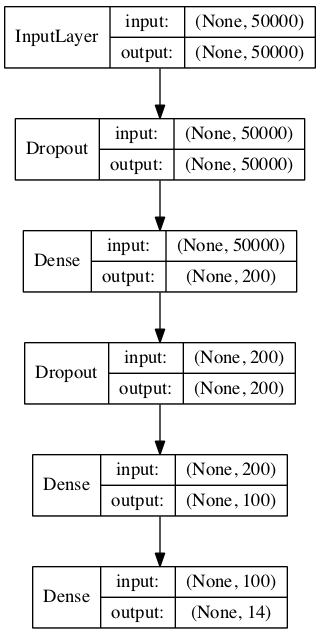
\includegraphics[height=0.3\textheight]{img/bow_nn}
	\caption{Feed-forward NN architecture for $50000$ words in vocabulary}
	\label{fig:bow_nn_architecture}
\end{figure}

\begin{figure}[h]
	\centering
	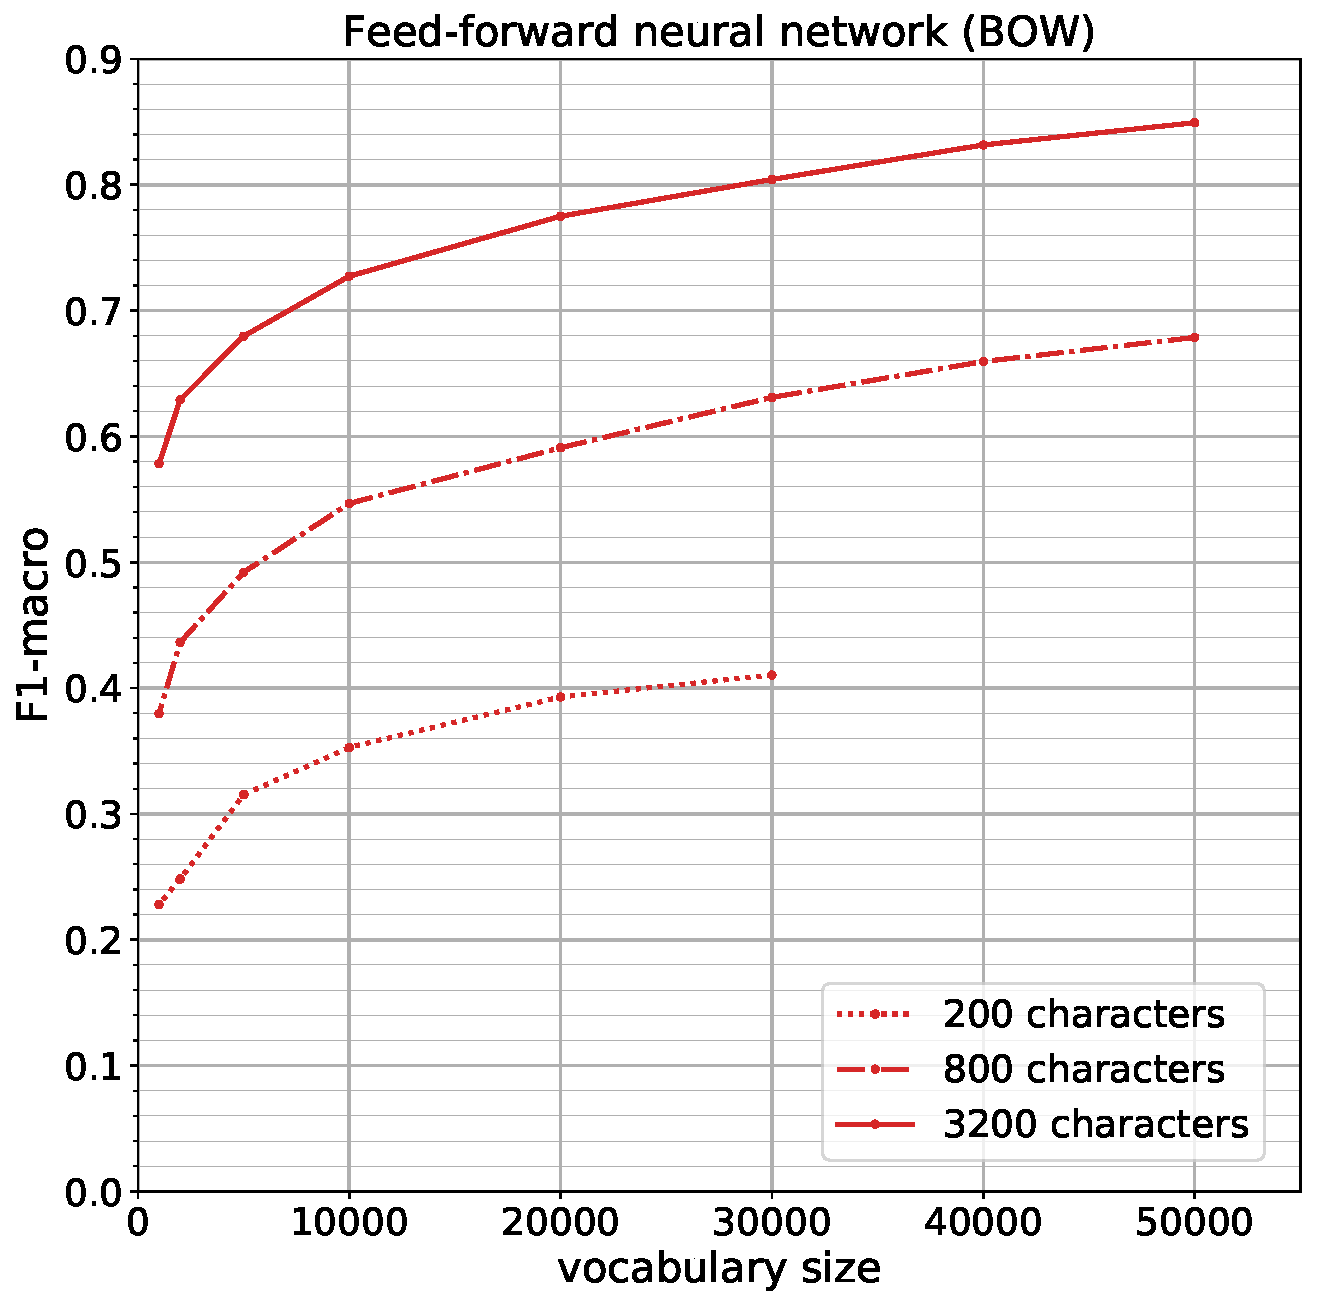
\includegraphics[height=0.3\textheight]{img/05_bow_nn}
	\caption{BOW with feed-forward NN classifier.}
	\label{fig:bow_nn}
\end{figure}


\begin{table}[h]
	\centering
	\begin{tabular}{|l|r|r|}\hline
		Document length (vocabulary size) & F1-macro score & Accuracy \\
		\hline
		$200$ chars  &  $0.410$   & $0.429$   \\
		$800$ chars  &  $0.679$   & $0.680$   \\
		$3200$ chars &  $0.849$   & $0.850$   \\
		\hline
	\end{tabular}
	\caption{Best performance of \textbf{feed-forward NN on binary BOW} for each document length.}
	\label{tbl:bow_nn}
\end{table}

\subsection{Tf-Idf}
Until now, the feature vector for each document was binary. Nevertheless, it performed quite decent. In the following, we represent documents as tf-idf vectors utilizing both the frequency of each word in the given document and the word overall frequency in the training corpus.

To compare with the binary approach, we applied Logistic Regression on top of \textit{Tf-Idf} vectors. Accuracy and F1-scores for all document lengths are shown in \cref{tbl:tfidf}. \cref{fig:05_tfidf} shows that \textit{Tf-Idf} can make use of extra words in the vocabulary as the score for all three document lengths is increasing with the size of vocabulary.

\begin{table}[h]
	\centering
	\begin{tabular}{|l|r|r|}\hline
		Document length (vocabulary size) & F1-macro score & Accuracy \\
		\hline
		$200$ chars  &  $0.395$   & $0.418$   \\
		$800$ chars  &  $0.663$   & $0.664$   \\
		$3200$ chars &  $0.836$   & $0.829$   \\
		\hline
	\end{tabular}
	\caption{Best performance of \textbf{logistic regression} on \textbf{tf-idf} for each document length.}
	\label{tbl:tfidf}
\end{table}

Similarly to the logistic regression on binary BOW, the regularization parameter $\alpha$ decreased with increasing size of vocabulary. The optimal $\alpha$ value for the best models of each document lengths turned at to be the same -- $10 ^{-6}$.

\begin{figure}[h]
	\centering
	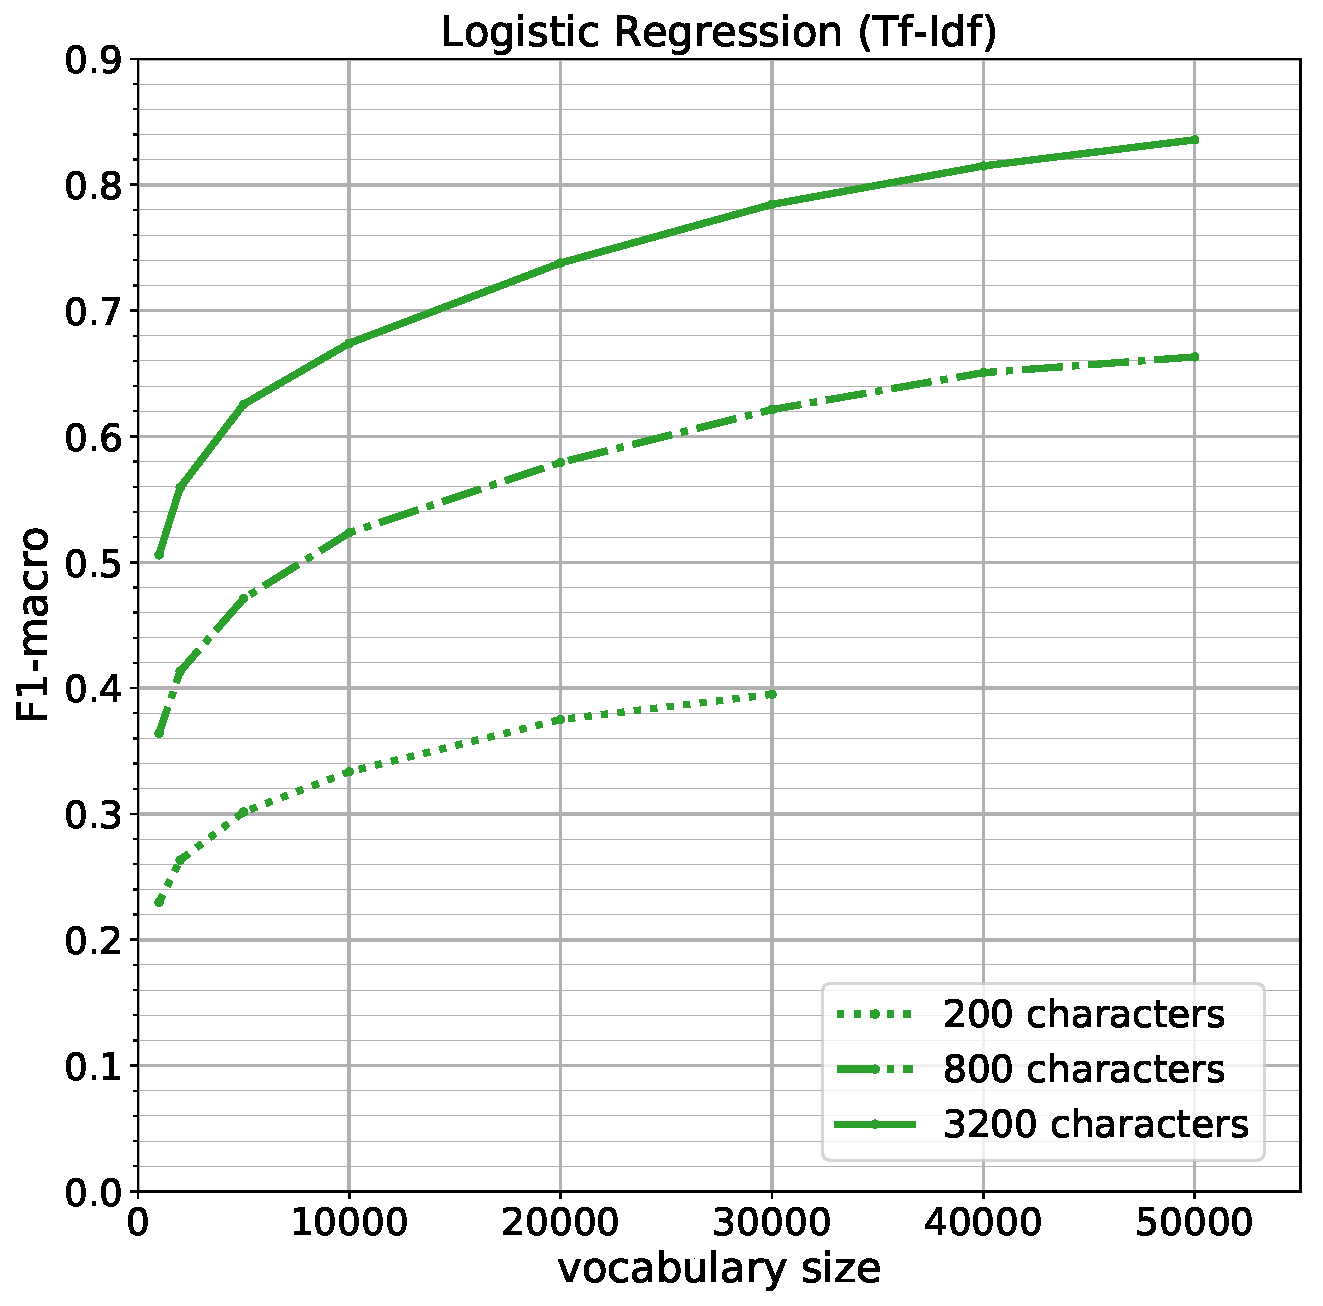
\includegraphics[height=0.3\textheight]{img/05_tfidf}
	\caption{F1-macro score comparison for Logistic Regression on Tf-Idf weighted vectors.}
	\label{fig:05_tfidf}
\end{figure}




\subsection{Summary BOW}

All in all, the score improved with growing vocabulary size for all algorithms and document lengths. For all three document lengths, neural network performed the best out of all algorithms, slightly better than logistic regression on tf-idf. Logistic regression on tf-idf performed better than on binary BOW and the gap increased with growing size of vocabulary. It is probably caused by tf-idf boosting the rare words\footnote{words not in top $10000$ most common words in the corpus} that might be defining the genre.\footnote{For example the word \textit{asteroid} occurred $54$ times in science fiction genre and never in any other genre.}

The Naive Bayes classifier performed the worst out of the tested algorithms. It performed very similar to other algorithms on short documents -- only $0.014$ worse than logistic regression on binary BOW. However, for longer documents, it could not predict genres as good as other algorithms -- falling behind the logistic regression on binary BOW by $0.08$ for middle-length documents and $0.12$ for long documents.

\cref{tbl:bow_comparison} shows the comparison of all algorithms and document lengths. The neural net reached F1-score of $0.849$ and accuracy $0.850$. The logistic regression on tf-idf performed was worse only by $0.013$ which is negligible given a lot higher training complexity and space needed to fit and store the neural net.

\begin{table}[h]
	\centering
	\begin{tabular}{|l|r|r|r|r|}\hline
		Document length & Naive Bayes & Log. reg. & Log. reg. (Tf-Idf) & NN \\
		\hline
		$200$ chars   & $ 0.360$  &  $0.374$  & $0.395$  &  $0.410$   \\
		$800$ chars   & $0.552$  &  $0.634$  & $0.663$  &  $0.679$   \\
		$3200$ chars  & $0.681$  &  $0.805$  & $0.836$  &  $0.849$   \\
		\hline
	\end{tabular}
	\caption{F1-score comparison of classifiers on BOW document representation for each document length.}
	\label{tbl:bow_comparison}
\end{table}


% \subsubsection{Short documents}

For short documents, the training set contained only $30000$ words after low occurrence words were filtered out. To improve the vocabulary quality, we tried out using the vocabulary fitted on the long documents with $3200$ characters expecting it to contain more relevant words and less noise as the vocabulary was fitted on $16$ times more text. However, contrary to our expectations, using this vocabulary actually slightly decreased the performance by about $0.02$ for both $800$ and $200$-character documents. 

The cause for this result is that when vocabulary was choosing top $n$ words based on frequency in the corpus, words with higher frequency in the corpus of long documents were preferred to those with high frequency in the training set of short documents. Therefore, the classification algorithms couldn't utilize the "better vocabulary".

\cref{fig:bow} shows comparisons of all BOW algorithms on each document length.


\begin{figure}
\centering
\begin{subfigure}[t]{.49\textwidth}
	\centering
	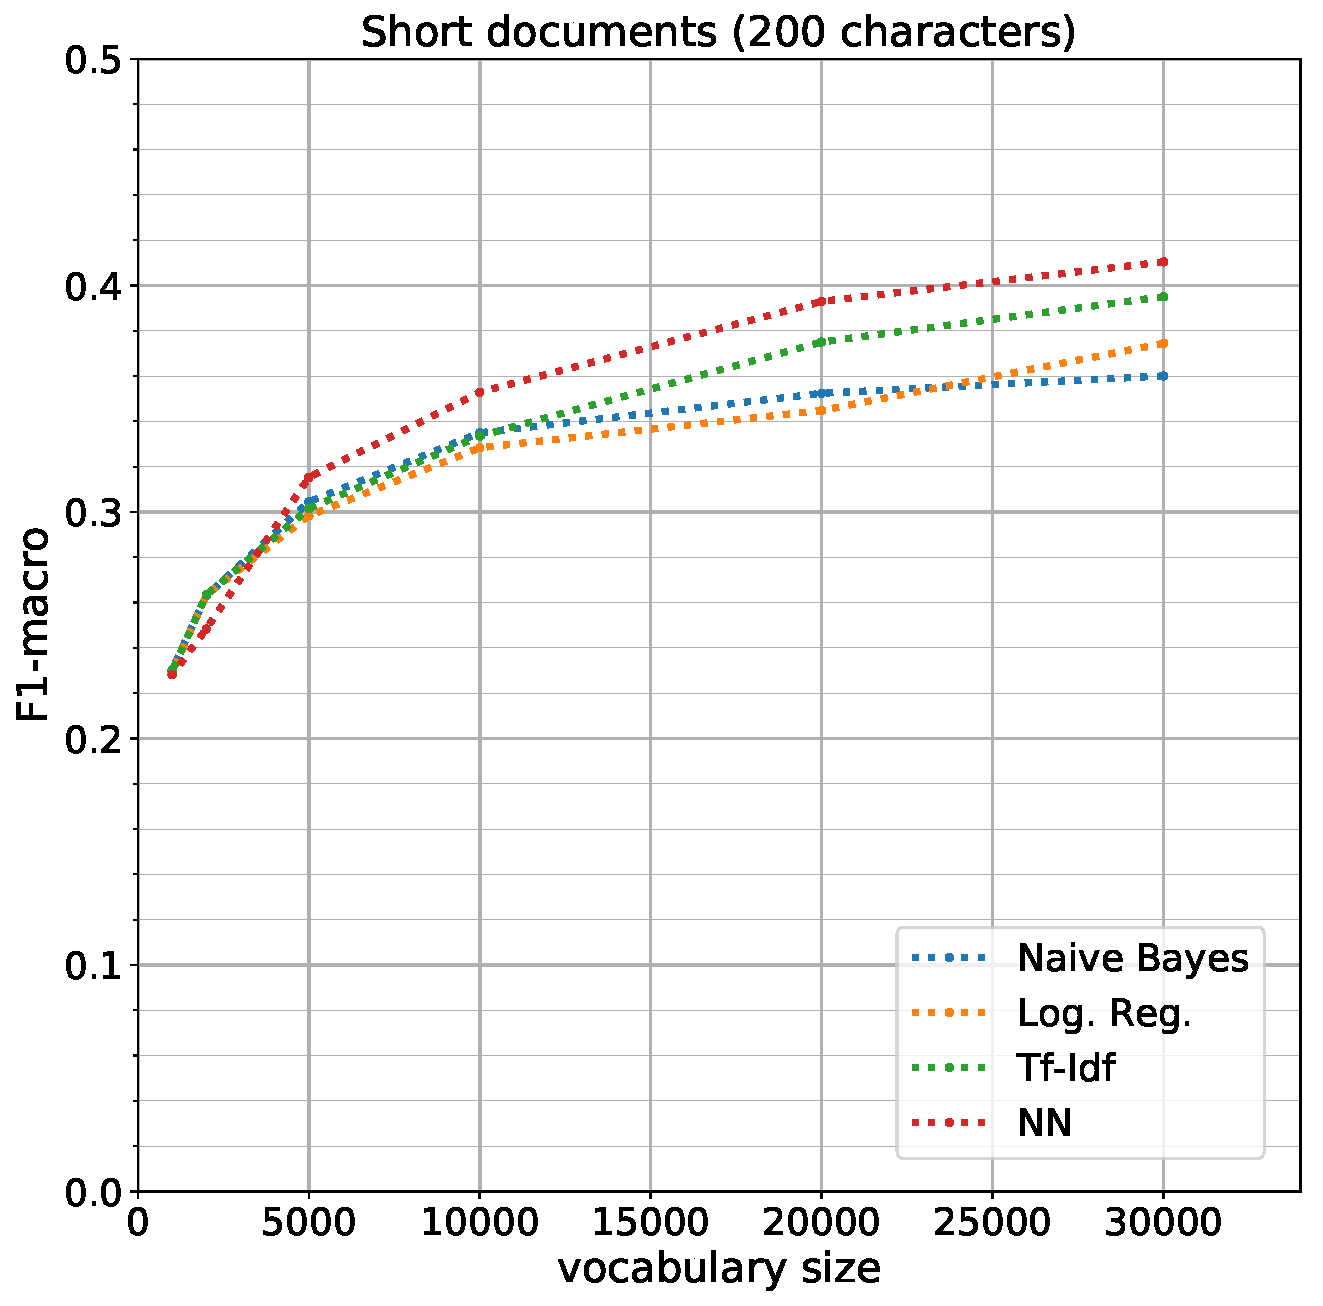
\includegraphics[width=0.99\linewidth]{img/05_bow_200}
	\caption{200 characters}
	\label{fig:05_bow_200}
\end{subfigure}%
\begin{subfigure}[t]{.49\textwidth}
	\centering
	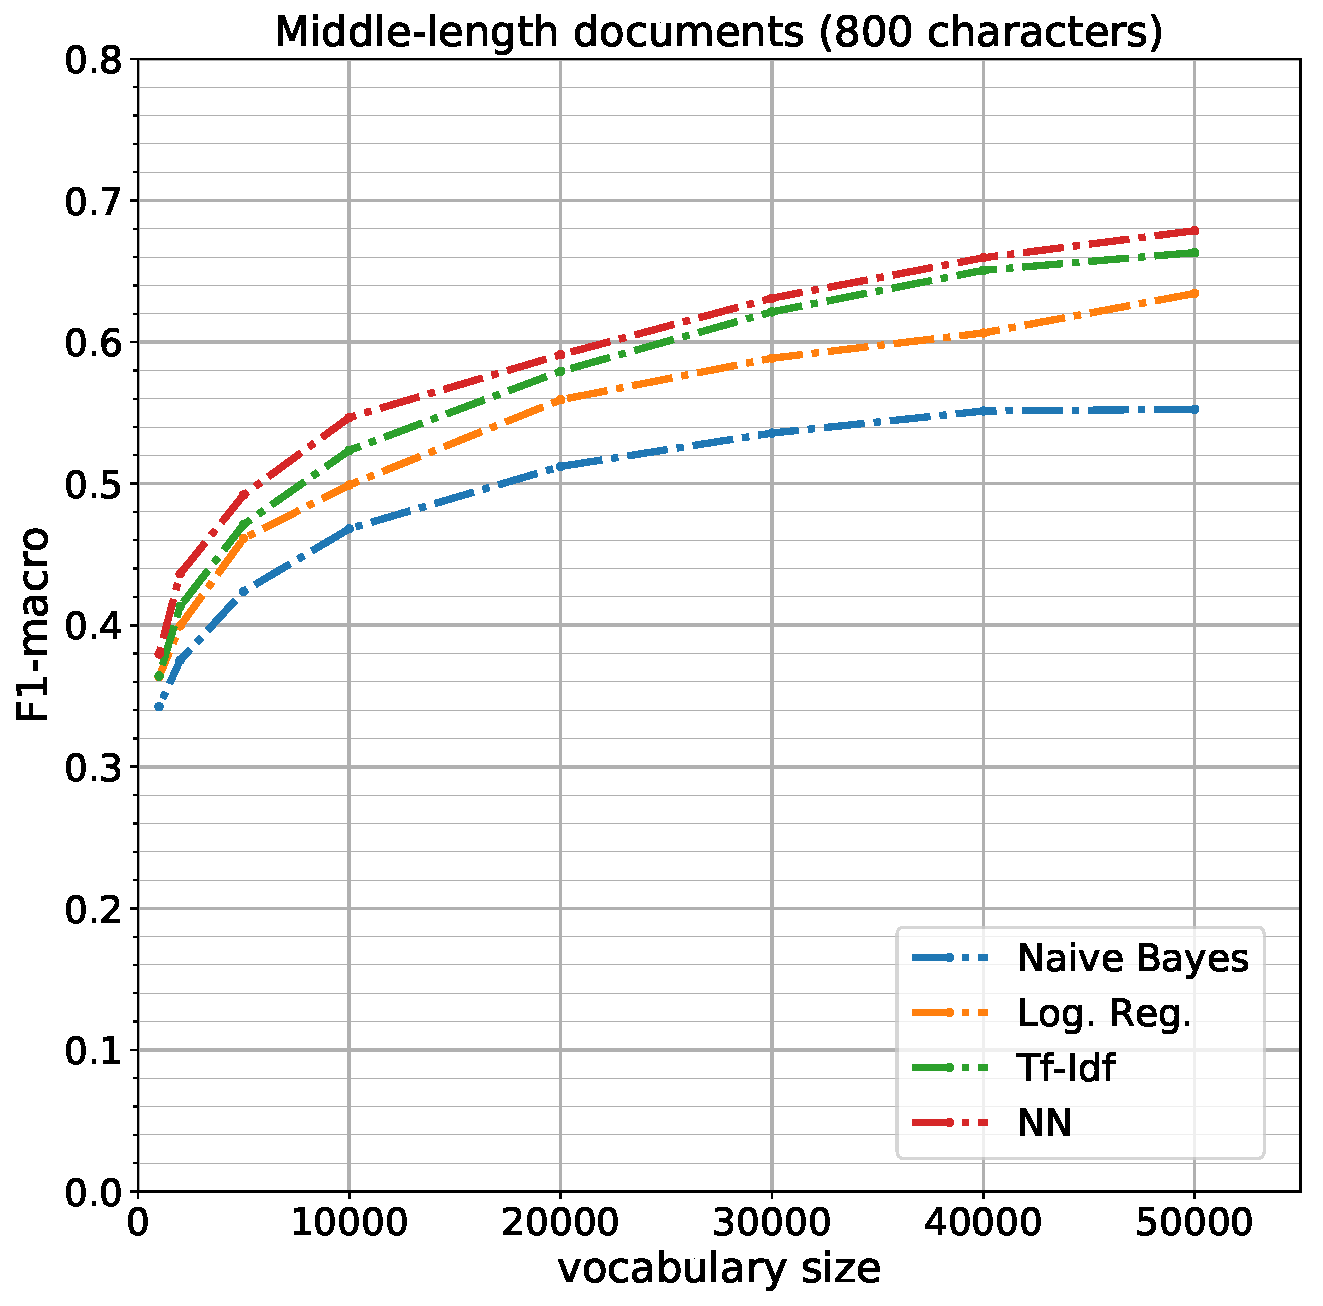
\includegraphics[width=0.99\linewidth]{img/05_bow_800}
	\caption{800 characters}
	\label{fig:05_bow_800}
\end{subfigure}

\begin{subfigure}[t]{.49\textwidth}
	\centering
	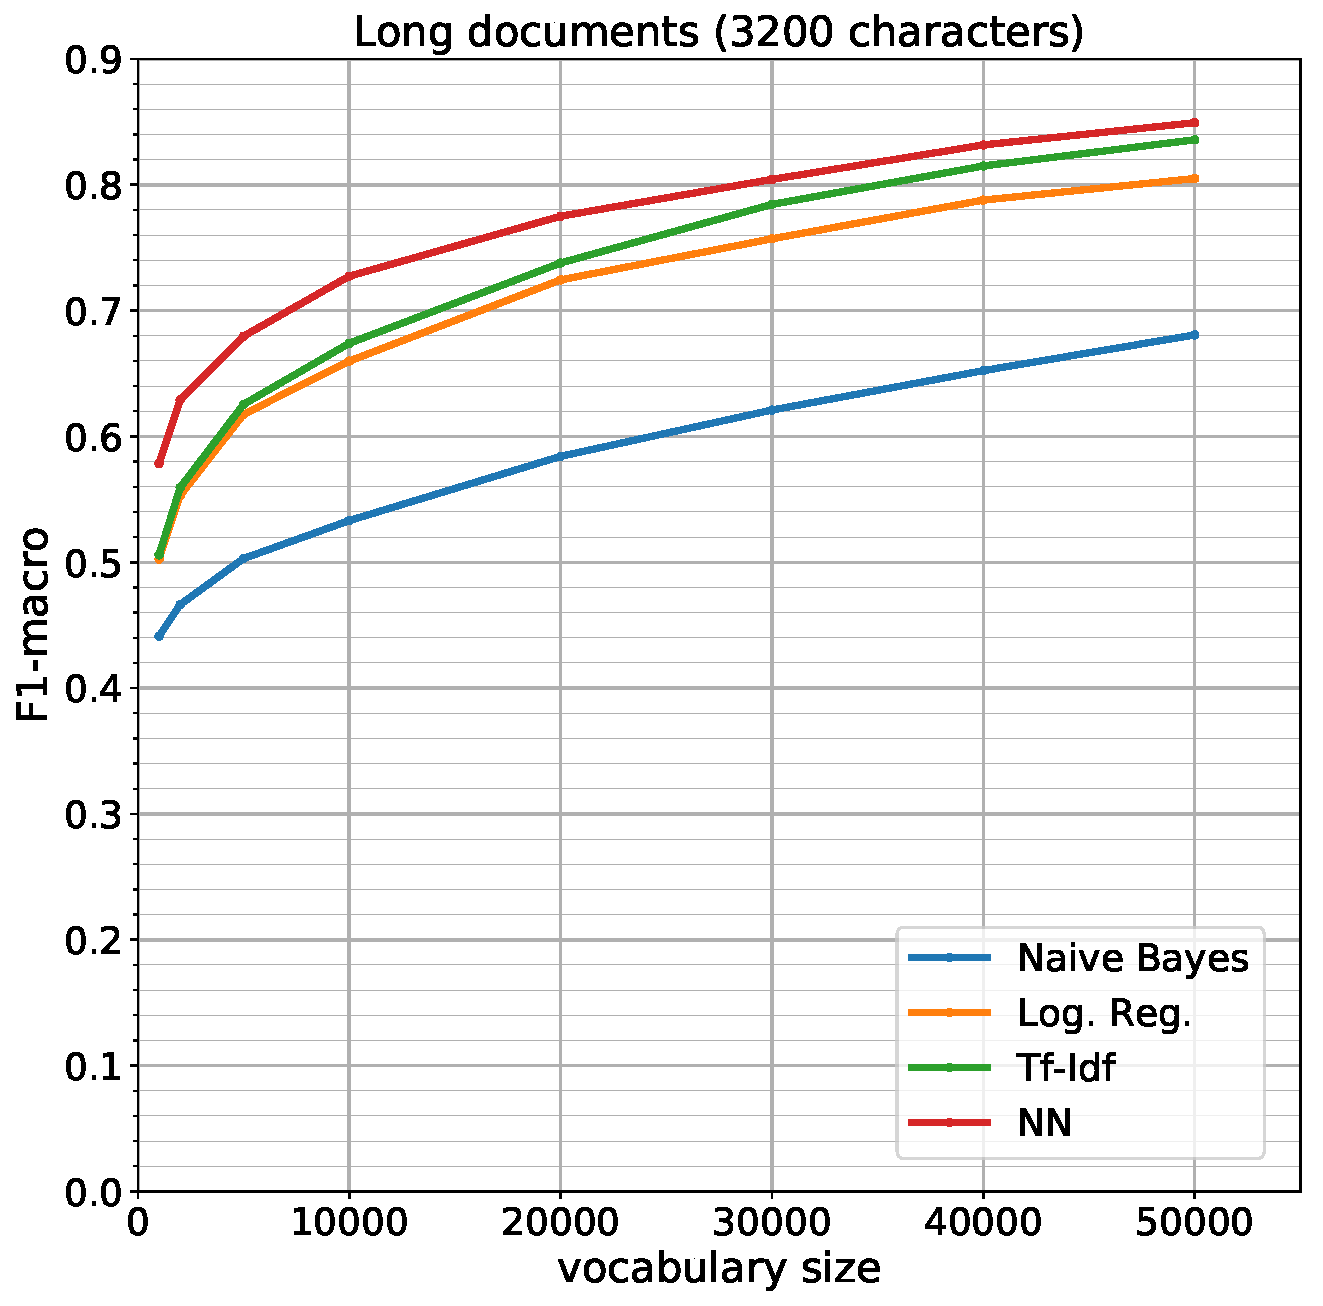
\includegraphics[width=0.99\linewidth]{img/05_bow_3200}
	\caption{3200 characters}
	\label{fig:05_bow_3200}
\end{subfigure}%

\caption{F1-macro score comparison for all BOW algorithms.}
\label{fig:bow}
\end{figure}



\begin{comment}
The reason for this might be that when using vocabulary created on other (even though larger) set, number of words in the shorter texts which are in that vocabulary is lower than when using vocabulary trained directly on documents itself. And fewer words in vocabulary means fewer information about the text (as words not in vocabulary are ignored and skipped), hence worse score.
\end{comment}

%\subsubsection{Medium-length documents}

%\cref{fig:05_bow_800}


%\subsubsection{Long documents}

%\cref{fig:05_bow_3200}



%%%%%%%%%%%%%%%%%%%%%%%%%%%%%%%%%%
%%%%%%%%%%%%%%%%%%%%%%%%%%%%%%%%%%
%%%%%%%%%% DOC2VEC  %%%%%%%%%%%%%%
%%%%%%%%%%%%%%%%%%%%%%%%%%%%%%%%%%
%%%%%%%%%%%%%%%%%%%%%%%%%%%%%%%%%%

\section{Doc2vec}
In the next approach, documents are embedded into a space of several hundred dimensions using \textit{doc2vec}. This representation is a lot smaller and compacter than the previous BOW approach where documents were represented by vectors with up to $50000$ dimensions.

For the document classification, we used similarity metrics to find most similar documents (kNN) or most similar genre vector. Apart from those,  logistic regression and simple neural network with one hidden layer containing $50$ neurons were used.

The training of doc2vec was done using the \textit{gensim}\cite{gensim} module for python and a big hyperparameter search had to be done to make the approach work for our task. The main parameters we had to tune were:

\begin{itemize}
  \item \textit{dimension} of the vectors
  \item choosing between \textit{dbow} and \textit{dm} architecture
  \item \textit{window size}
\end{itemize}

\subsection{Hyperparameter tuning}
For the initial parameter setting, we adopted the parameters from J. H. Lau and T. Baldwin - An Empirical Evaluation of doc2vec with Practical Insights into Document Embedding Generation\cite{doc2vec_params}. They also report improvement when initializing the doc2vec model with word embeddings trained on bigger corpus.

In order to choose the right hyperparameters, we have to find a way to compare trained doc2vec models. As we train not only document vectors but also genre vectors, the quality can be estimated by comparing the inferred documents from the validation set with the genre vectors and computing how often was the vector of the correct genre the most similar one out of all $14$ genre vectors in terms of cosine similarity.

%Models are compared and selected based on "nearest genre classifier".

\subsubsection{Distributed BOW (DBOW) vs. Distributed Memory (DM)}
Le \& Mikolov, the original authors of the Paragraph vector\cite{doc2vec}, 
propose two architectures.

The first one is Distributed Memory where the task is to predict a missing word from the window given the context (surrounding words) and the paragraph vector.

The second architecture is is Distributed bag of words where the net is trained to predict words in a small window given the document vector.

Le \& Mikolov report distributed memory version to perform better.\cite{doc2vec} However, Lau and Baldwin\cite{doc2vec_params} as well as the creators of gensim\cite{gensim} observed the distributed BOW version to obtain better results.

In our experiments, we join the latter as the Distributed BOW version reaches $0.05$ to $0.1$ better score on the task of genre classification than the Distributed Memory architecture.

The following hyperparameter discussion focuses then on the DBOW doc2vec.

\subsubsection{Vector dimension}
Le \& Mikolov used in the original work vectors with $400$ dimensions.\cite{doc2vec}, Lau and Baldwin chose $300$ dimensions.\cite{doc2vec_params}

For our task, number of dimensions between $300$ and $400$ worked the best as well. The performance did not improve for vector sizes bigger than $500$ and for less than $200$ dimensions, the performance started decreasing.

\subsubsection{Window size}
Discuss impact of window size on the quality of vectors for each length.
\subsubsection{Including genre vectors}
\begin{itemize}
	\item way better performance when including genre vectors
	\item tried also to add original book vector (as multiple documents come from the same book) but didn't improve genre prediction
	\item as shown later, it not only improves document embeddings but also enables us to use the nearest genre vector of a text as a decent prediction
\end{itemize}

\subsubsection{Pre-trained word embeddings}
As mentioned before, Lau and Baldwin\cite{doc2vec_params} report improvement when using pre-trained word vectors. For our task, using $GloVe$ vectors with $300$ dimensions trained on Wikipedia improved the score. The improvement was more significant for predictions based on short documents. That comes as no surprise as short documents contain less data to train a good word-embedding than longer documents..

\subsubsection{Learning rate $\alpha$}
The default training rate$ \alpha$ in gensim is $0.025$ which turned out to be too large for our setting. Best working alphas we observed were between $0.0075$ and $0.015$.
\begin{comment}
	And multiplying alpha by 4/5 or 9/10 at the end of every iteration
\end{comment}

\subsubsection{Document shuffling}
Another thing that improves the document vector quality is reshuffling of training samples at the beginning of each epoch. Reshuffling, however considered as a standard for neural net training, is not supported by gensim\footnote{At least not at the time of writing this text -- June 2018} and has to be done manually. Doing so constantly improves the score by couple of percent points.

\subsubsection{Vector inference for new documents}
\begin{itemize}
	\item $3$ infer steps instead of default $5$ in gensim works better
	\item as inferring is not deterministic, nearest genre classifier works best if we infer the vector multiple times (ca 10) and make a majority vote
\end{itemize}

\subsection{Similarity Cosine similarity with genre vectors}

The first classifier we applied after training the doc2vec representation, was \textit{Nearest genre vector}. It simply chooses the nearest genre vector to a document using cosine similarity between the vectors.

\begin{itemize}
	\item show table of performance with/wo genre and book vectors and w/wo GloVe embeddings
	\item $O(1)$ time and space, no training needed
\end{itemize}

Do multiple infers and majority vote - improves ca. $2\ \%$.

3 infer steps instead of 5 - default in gensim

\subsection{K most similar books (KNN)}

KNN - slow, cosine sim. better than eucl.

For $k = 10$, the performance was $.809$

\subsection{Logistic Regression}
Logistic Regression on document vectors ($200$ dimensions) performed worse than when using BOW representation.

\begin{table}[h]
	\centering
	\begin{tabular}{|l|r|r|}\hline
		Document length & F1-macro score & Accuracy \\
		\hline
		$200$ chars   &  $0.261$   & $0.316$   \\
		$800$ chars   &  $0.430$   & $0.468$   \\
		$3200$ chars  &  $0.551$   & $0.580$   \\
		\hline
	\end{tabular}
	\caption{Best performance for \textbf{doc2vec} ($200$ dimensions) representation with \textbf{Logistic Regression} classifier.}
	\label{tbl:doc2vec_logreg}
\end{table}

\subsection{Linear SVM}
\begin{itemize}
	\item Implemented as stochastic gradient descent with hinge loss.
	\item Linear SVM marginally worse than logistic regression.
	\item RBF was not better plus the kernel has to be precomputed which is very expensive for almost $200000$ training points.
\end{itemize}

\section{Error analysis}
Select few documents for logreg tf-idf and logreg/cosine sim for doc2vec that were confidently assigned to another genre and look at their text. Does it make sense for a human that they were misclassified?

\section{Combined approach}
Taking softmax probabilities of 3 classifiers
\begin{itemize}
	\item logreg on tfidf
	\item logreg on doc2vec
	\item nearest genre classifier
\end{itemize}
Running neural net with $20$ hidden neurons on top of that.
\begin{itemize}
	\item reaches best result
	\item impractical, more of a theoretic result
\end{itemize}
%Mention Random Forest, SVM and Annoy weren't better?
















\begin{comment}

\subsection{Annoy}
As the train set contains almost $200000$ documents, nearest neighbour algorithms running in linear time and space, such as \textit{K-Nearest Neighbours}, are impractical and expensive to use. Therefore, we used one of the approximate nearest neigbour algorithms - \textit{Annoy}. We introduced Annoy classifier which wraps Annoy algorithm into a proper classifier. 

The classifier finds $k$ nearest neighbours and weights the classes of the $k$ neighbours using given neighbourhood weighting.

Discuss Annoy details:
\begin{itemize}
  \item number of trees - The more trees, the more accurate but slower is the classification.
  \item k neighbours - Grid search on validation set for best k
  \item distance metric - Grid search on validation set for best distance metric
  \item neighbourhood weighting - Grid search on validation set for best neigbourhood weighting (How to aggregate the k-nearest neighbours)
\end{itemize}

Annoy performed quite well on the long documents while the performance on the shorter documents was slightly lower as shown in \cref{tbl:annoy}.

\begin{table}[h]
	\centering
	\begin{tabular}{|l|r|r|}\hline
		Document length & F1-macro score & Accuracy \\
		\hline
		$200$ chars   &  $0.235$   & $0.281$   \\
		$800$ chars   &  $0.492$   & $0.505$   \\
		$3200$ chars  &  $\textbf{0.813}$   & $0.810$   \\
		\hline
	\end{tabular}
	\caption{Best performance for \textbf{doc2vec} ($500$ dimensions) representation with \textbf{Annoy Classifier} .}
	\label{tbl:annoy}
\end{table}



\section{CNN}
\begin{itemize}
  \item Using pretrained GloVe embedding vectors (dimensions $50$, $100$, $200$ or $300$)
\end{itemize}

Architecture inspired by Yoon Kim\cite{yoon_kim}. An example of Convolutional Neural Network for long documents padded to $500$ words using GloVe word embeddings with $100$ dimensions is shown in \cref{fig:cnn}.

\begin{figure}[h]
	\centering
	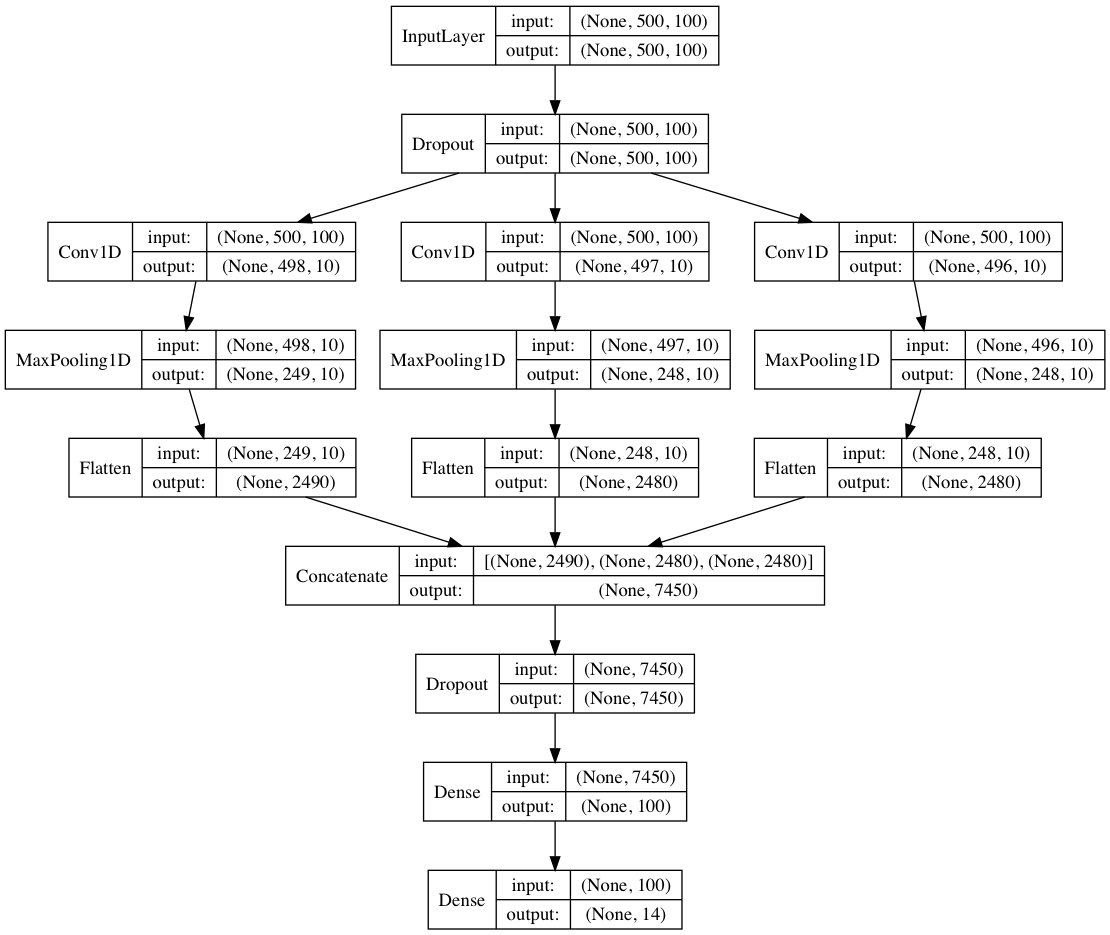
\includegraphics[height=0.35\textheight]{img/cnn}
	\caption{CNN with input consisting of $500$ words represented by $100$ dimensional GloVe vectors.}
	\label{fig:cnn}
\end{figure}

The best results are shown in \cref{tbl:cnn}.
\begin{table}[h!]
	\centering
	\begin{tabular}{|l|l|l|r|}\hline
		Document length & padding length & vector dim. & F1-macro score\\
		\hline
		$200$ chars   & 50 &  300 & $0.288$   \\
		$800$ chars   & 200 & 100 & $0.410$   \\
		$3200$ chars  & 500 & ? & $?$    \\
		\hline
	\end{tabular}
	\caption{Best performance for \textbf{CNN}.}
	\label{tbl:cnn}
\end{table}

\end{comment}

\textbf{TODO:} Put confusion matrix for each classifier and discuss.



\chapter{Insights}

\section{Typical Words}

\subsection{Tf-Idf}
How did we define typical words for tf-idf:
\begin{itemize}
	\item define tf-idf genre vectors by averaging all document vectors of given genre (on training set)
	\item compute an average tf-idf vector of the whole training set
	\item subtract the average vector from each genre vector
	\item The most important words are those with highest scores
	\item Based on desired output, filter out too short words (having only two characters) and rare words (e.g. keep only those which occurred at least in $0.5\ \%$ of documents)
	\item investigate words with highest and lowest variance in tf-idf coefficient among the $14$ genre vectors
\end{itemize}

\subsection{Doc2Vec}
\begin{itemize}
	\item look at words most similar to the trained genre vectors
\end{itemize}

As we trained also word embeddings for the doc2vec model, we can look at similarities between a document and a word. To get a representative vector of a given genre, we average all vectors of that genre. 

Next, we compute dot products between the genre vector and all words in the vocabulary. As we want to get representative words of the genre, we filter out uncommon words which occured in less than $0.5\ \%$ of all documents. We also focus only on words consisting of at least 4 letters, as shorter words seem to have higher similarity to all documents in general when computed based on dot product. \cref{fig:typical_words_genre} shows a word cloud of most typical words for \textit{detective and mystery stories}, \textit{science fiction} and \textit{western stories}.


When using different similarity metrics, the typical words didn't seem too meaningful. For \textit{cosine similarity}, due to normalization, shorter words tend to be much more similar to all documents in general than other words. For euclidean metric, All genres gave same typical words.


\section{Document similarity}
Choose a document and find most similar documents. Look at accuracy @ 1, 3, 5, 10 documents for the following:
\begin{itemize}
	\item Are they part of the same book? - 
	\item Same author?
	\item Same genre?
\end{itemize}


\begin{figure}[h]
	\centering
	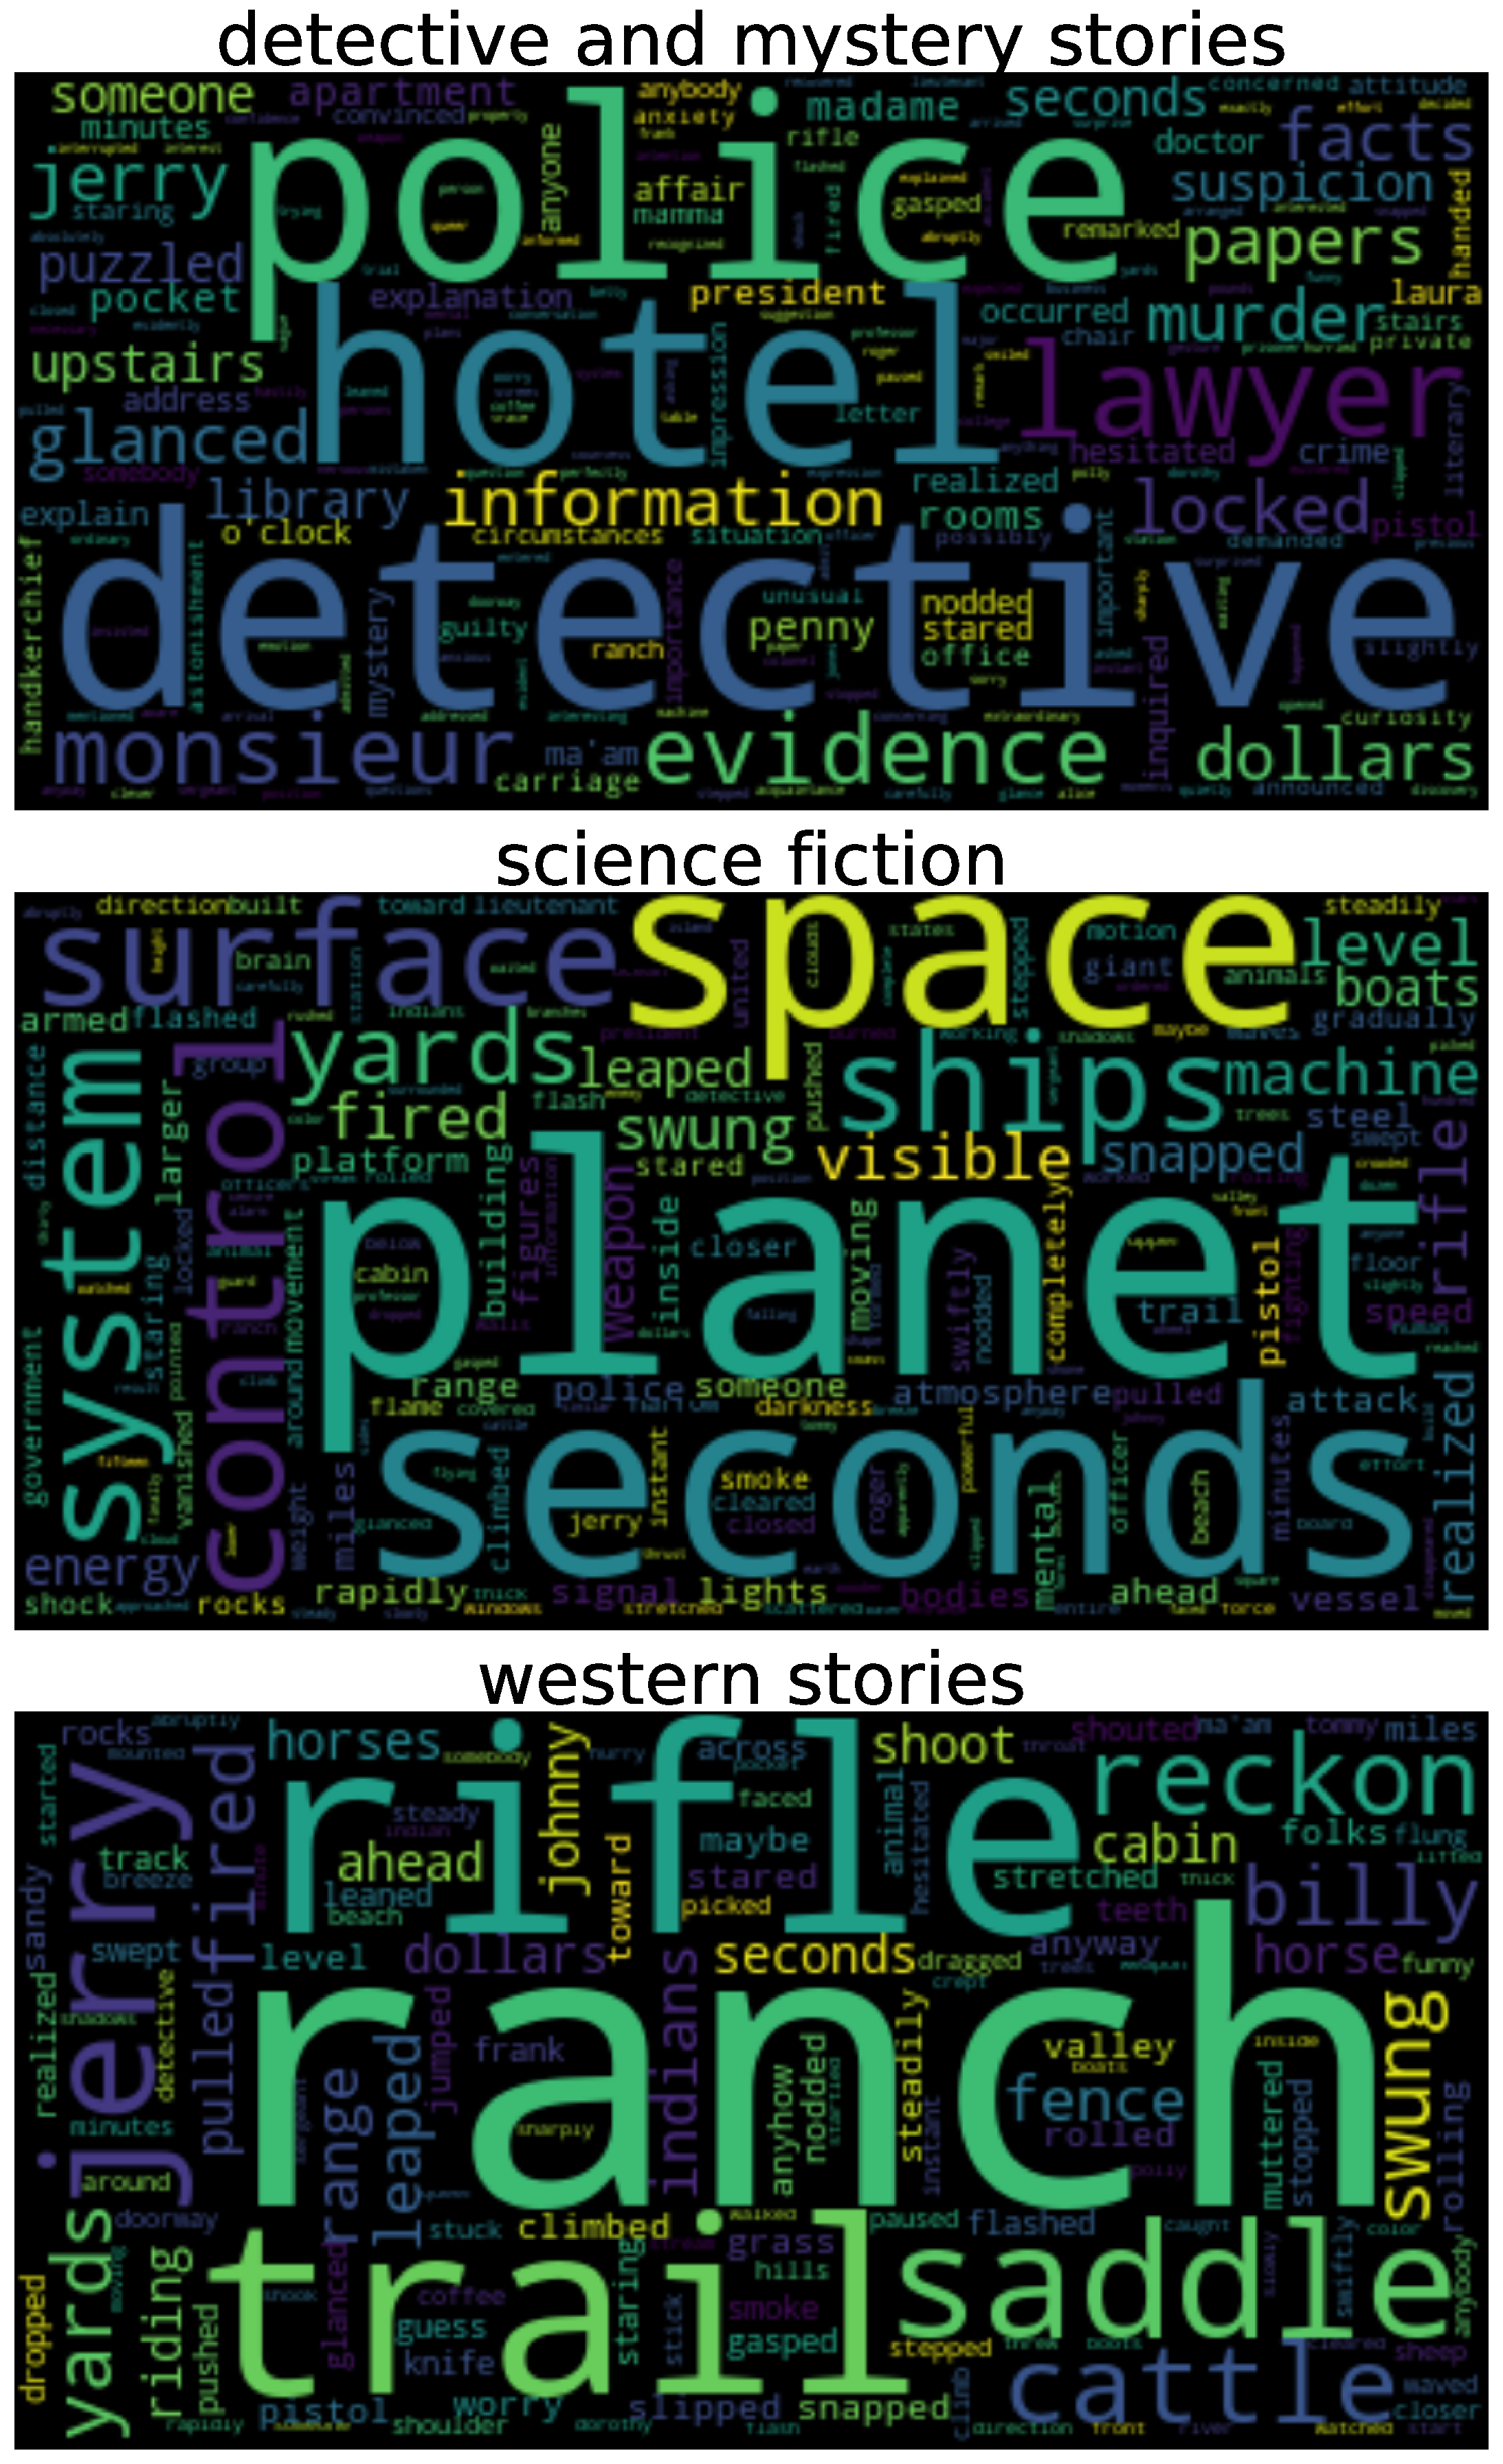
\includegraphics[height=0.6\textheight]{img/06_typical_words_genre}
	\caption{Typical words for \textit{detective and mystery stories}, \textit{science fiction} and \textit{western stories} based on doc2vec and dot product document-word similarity.}
	\label{fig:typical_words_genre}
\end{figure}

\section{Visualizing document vectors}
To visualize documents in 2D, we transformed the document vectors to $2$ dimensions using dimensionality reduction techniques. The final plot is made by t-SNE algorithm. However, as the convergence takes very long for large datasets, we first run PCA and transformed the data to $50$ dimensions and run t-SNE on those.

\chapter{Implementation}
Describes details of the implementations. We used gensim\cite{gensim}.
\begin{itemize}
  \item Text classifiers deployed to heroku 
  \subitem https://book-genres-prediction.herokuapp.com
  \item Which algorithm is used?
  \item Deploy / implementation details on technologies etc. $\cdots$
\end{itemize}

\chapter{Summary}

\section{Summary and Conclusions}

\begin{itemize}
    \item Looked at text genre classification into $14$ classes of documents of sizes $200$, $800$ and $3200$ characters
    \item The classification accuracy grew with increasing length of the documents indicating the algorithms had difficulties to recognize genre from only a short snippet.
    \item Bigger gap in performance between documents with $200$ and $800$ words than between $800$ and $3200$ words.
    \item Feed-forward neural net on feature vectors outperforms logistic regression but not by much\dots
    \item Provided insights into what is typical for each genre (typical words)
    \item Deployed couple of classifiers to heroku with web interface
\end{itemize}

\section{Future Work}


%\include{epilog}

%%% Bibliography
%%% Bibliography (literature used as a source)
%%%
%%% We employ bibTeX to construct the bibliography. It processes
%%% citations in the text (e.g., the \cite{...} macro) and looks up
%%% relevant entries in the bibliography.bib file.
%%%
%%% The \bibliographystyle command selects, which style will be used
%%% for references from the text. The argument in curly brackets is
%%% the name of the corresponding style file (*.bst). Both styles
%%% mentioned in this template are included in LaTeX distributions.

% \bibliographystyle{plainnat}    %% Author (year)
\bibliographystyle{unsrt}     %% [number]

\renewcommand{\bibname}{Bibliography}

%%% Generate the bibliography. Beware that if you cited no works,
%%% the empty list will be omitted completely.

\bibliography{bibliography}

%%% If case you prefer to write the bibliography manually (without bibTeX),
%%% you can use the following. Please follow the ISO 690 standard and
%%% citation conventions of your field of research.

% \begin{thebibliography}{99}
%
% \bibitem{lamport94}
%   {\sc Lamport,} Leslie.
%   \emph{\LaTeX: A Document Preparation System}.
%   2nd edition.
%   Massachusetts: Addison Wesley, 1994.
%   ISBN 0-201-52983-1.
%
% \end{thebibliography}


%%% Figures used in the thesis (consider if this is needed)
%\listoffigures

%%% Tables used in the thesis (consider if this is needed)
%%% In mathematical theses, it could be better to move the list of tables to the beginning of the thesis.
%\listoftables

%%% Abbreviations used in the thesis, if any, including their explanation
%%% In mathematical theses, it could be better to move the list of abbreviations to the beginning of the thesis.
%\chapwithtoc{List of Abbreviations}

%%% Attachments to the bachelor thesis, if any. Each attachment must be
%%% referred to at least once from the text of the thesis. Attachments
%%% are numbered.
%%%
%%% The printed version should preferably contain attachments, which can be
%%% read (additional tables and charts, supplementary text, examples of
%%% program output, etc.). The electronic version is more suited for attachments
%%% which will likely be used in an electronic form rather than read (program
%%% source code, data files, interactive charts, etc.). Electronic attachments
%%% should be uploaded to SIS and optionally also included in the thesis on a~CD/DVD.
%%% Allowed file formats are specified in provision of the rector no. 72/2017.
\iffalse
\appendix
\chapter{Attachments}

\section{First Attachment}
\fi

\openright
\end{document}
